\chapter{Análisis}

\section{Análisis de los Sensores}

El análisis de los sensores constituye un paso esencial en el desarrollo de este proyecto. El objetivo principal de esta actividad es evaluar y comprender las especificaciones técnicas de los sensores disponibles en el mercado que serán utilizados en la WSN.\\
Durante este análisis, se examinarán aspectos clave de los sensores, como su precisión, rango de medición, resolución, consumo de energía, frecuencia de muestreo y capacidad de transmisión de datos. Además, se considerarán las condiciones ambientales en las que operarán los sensores, como la temperatura, la humedad y la resistencia a la intemperie, para asegurar su idoneidad en el entorno de monitoreo.\\
El resultado de esta actividad será un informe detallado que incluirá una comparación exhaustiva de los sensores analizados, resaltando sus ventajas y limitaciones. Este informe servirá como base para la selección de los sensores más apropiados en función de los requisitos específicos del proyecto, asegurando así la adquisición de equipos que se ajusten de manera óptima a los objetivos de monitoreo y a las condiciones del entorno.

\noindent Aspectos clave a evaluar en los sensores:

\begin{enumerate}
\item \textbf{Precisión:} La precisión de los sensores es fundamental, ya que determina cuán cercanas son las mediciones a los valores reales. Se analizará cuán exactos son los sensores en la detección de variables específicas, como temperatura, humedad, presión, o cualquier otro parámetro relevante para el monitoreo de la especie animal.
\item \textbf{Rango de Medición:} El rango de medición define los valores mínimos y máximos que un sensor puede detectar con precisión. Se evaluará si el rango de medición de los sensores es adecuado para capturar las variaciones esperadas en los datos del entorno de monitoreo, teniendo en cuenta las características del animal y su hábitat.
\item \textbf{Resolución:} La resolución se refiere a la capacidad del sensor para distinguir pequeñas diferencias en los datos. Se examinará cuán fina es la resolución de los sensores, lo que es especialmente importante cuando se requiere una alta sensibilidad para detectar cambios sutiles en las condiciones ambientales.
\item\textbf{Consumo de Energía:} El consumo de energía de los sensores es esencial para garantizar la durabilidad de la WSN y minimizar la necesidad de cambios frecuentes de batería. Se analizará cuánta energía consumen los sensores durante la adquisición de datos y en modo de espera, y se buscarán soluciones de eficiencia energética.
\item\textbf{Frecuencia de Muestreo: }La frecuencia de muestreo indica con qué regularidad los sensores capturan y transmiten datos. Se determinará la frecuencia de muestreo óptima para obtener datos relevantes sin generar una carga innecesaria en la red y los drones.
\item \textbf{Capacidad de Transmisión de Datos:} La capacidad de transmisión de datos se relaciona con la velocidad y la distancia a la que los sensores pueden enviar información a la estación base. Se considerará si los sensores pueden transmitir datos de manera eficiente y oportuna, especialmente cuando se requiere una transmisión en tiempo real.
\item \textbf{Condiciones Ambientales:} Se evaluará la capacidad de los sensores para operar en las condiciones ambientales específicas del hábitat de la especie animal. Esto incluye la resistencia a la intemperie, la capacidad de funcionar en entornos húmedos o polvorientos, y la tolerancia a temperaturas extremas.
\end{enumerate}

\subsection{Comparación de Sensores}
En la búsqueda de los sensores adecuados para este proyecto, es esencial comprender las capacidades y limitaciones de las diferentes opciones disponibles. A continuación, se presenta una descripción técnica detallada de los sensores que se consideran relevantes para el sistema de monitoreo de especies en peligro de extinción. Cada uno de estos sensores desempeña un papel único en la recopilación de datos. Esta comparación exhaustiva se realiza para tomar decisiones informadas al momento de seleccionar los sensores más apropiados a las necesidades del proyecto y al entorno de monitoreo en el que se operará.
\begin{itemize}
    

\item \textbf{Humedad:} Los sensores de humedad miden el contenido de humedad en el aire o el suelo. Utilizan componentes sensibles a la humedad, como higroscópicos, para convertir la humedad en señales eléctricas. Estos sensores son económicos y eficientes en cuanto al consumo de energía. Son adecuados para entornos donde la humedad ambiental es un factor relevante para el comportamiento de las especies, como en estudios de hábitats acuáticos o de humedales \cite{75}.
\item \textbf{Temperatura:} Los sensores de temperatura registran la temperatura ambiente. Estos sensores están ampliamente disponibles y son económicos. Pueden utilizarse para monitorear las preferencias térmicas de las especies y detectar cambios de temperatura que puedan afectar su comportamiento \cite{76}.
\item \textbf{Sonido:} Los sensores de sonido capturan las vocalizaciones y otros sonidos ambientales. Son útiles para registrar el comportamiento de las especies que emiten vocalizaciones y para analizar la actividad acústica en el entorno. Sin embargo, la identificación precisa de las especies a menudo requiere análisis avanzados debido a la diversidad de sonidos en la naturaleza \cite{77}.
\item \textbf{Presión Atmosférica:} Los sensores de presión atmosférica miden la presión del aire y, a menudo, se utilizan para estimar la altitud. Son esenciales para vuelos de drones, ya que ayudan a determinar la altitud y la presión en diferentes alturas. Aunque no proporcionan información específica sobre las especies, son cruciales para la operación segura de drones en la atmósfera \cite{78}.
\item \textbf{Altitud:} Los sensores de altitud son necesarios para medir la altitud sobre el nivel del mar y la elevación en terrenos montañosos. Estos sensores son relevantes cuando se estudian especies que exhiben comportamiento altitudinal o en áreas montañosas. A menudo se utilizan en conjunto con otros sensores para obtener información precisa \cite{79}.
\item \textbf{GPS (Sistema de Posicionamiento Global):} Los dispositivos GPS proporcionan datos de ubicación precisos mediante la recepción de señales de satélites. Son fundamentales para la geolocalización de las especies y la recopilación de datos de movimiento. Sin embargo, consumen más energía en comparación con otros sensores y requieren una línea de visión directa con los satélites \cite{80}.
\item \textbf{Proximidad:} Los sensores de proximidad detectan la cercanía de objetos o animales a través de señales de infrarrojos, ultrasonidos u otros métodos. Son útiles para el monitoreo de trampas o la detección de la presencia de especies en áreas específicas. Sin embargo, tienen un alcance limitado y no proporcionan datos detallados sobre las especies en sí.\cite{81}
\item \textbf{Cámara Trampa:} Las cámaras trampa capturan imágenes discretas cuando se detecta movimiento. Son efectivas para la identificación visual de especies y su comportamiento. Requieren almacenamiento y procesamiento de imágenes, y pueden verse afectadas por condiciones de luz y clima \cite{82}.
\item \textbf{Imagen Multiespectral:} Los sensores de imagen multiespectral capturan datos en múltiples bandas del espectro electromagnético. Son útiles para analizar características ambientales, como la vegetación y la calidad del suelo. Sin embargo, son costosos y requieren sensores específicos, así como un manejo y análisis más complejos de los datos \cite{83}.
\end{itemize}

% Please add the following required packages to your document preamble:
% \usepackage{graphicx}
% Please add the following required packages to your document preamble:
% \usepackage{multirow}
% \usepackage{graphicx}
% Please add the following required packages to your document preamble:
% \usepackage{multirow}
% \usepackage{graphicx}
% Please add the following required packages to your document preamble:
% \usepackage{multirow}
% \usepackage{graphicx}
% Please add the following required packages to your document preamble:
% \usepackage{multirow}
% \usepackage{longtable}
% Note: It may be necessary to compile the document several times to get a multi-page table to line up properly
\begin{longtable}[c]{|c|l|}
\caption{Características específicas de los sensores de medición.}
\label{tab:my-table}\\
\hline
Sensor & \multicolumn{1}{c|}{Características} \\ \hline
\endfirsthead
%
\endhead
%
\hline
\endfoot
%
\endlastfoot
%
\multirow{7}{*}{Humedad} & Precisión:   ±2\% HR \\
 & Rango de Medición: 0\% a 100\%   HR \\
 & Resolución: 0.1\% HR \\
 & Consumo de Energía: Bajo   consumo \\
 & Frecuencia de Muestreo:   Ajustable \\
 & Capacidad de Transmisión:   Hasta 1 Hz \\
 & Condiciones Ambientales: -40°C   a 85°C \\ \hline
\multirow{7}{*}{Temperatura} & Precisión: ±0.5°C \\
 & Rango de Medición: -40°C a   125°C \\
 & 0.1\% HR: 0.1°C \\
 & Consumo de Energía: Bajo   consumo \\
 & Frecuencia de Muestreo:   Ajustable \\
 & Capacidad de Transmisión:   Hasta 1 Hz \\
 & Condiciones Ambientales: -55°C   a 125°C \\ \hline
\multirow{7}{*}{Sonido} & Precisión: Variable \\
 & Rango de Medición: Varía \\
 & 0.1°C: Variable \\
 & Consumo de Energía: Bajo   consumo \\
 & Frecuencia de Muestreo:   Ajustable \\
 & Capacidad de Transmisión: En   tiempo real \\
 & Condiciones Ambientales:   Sensible a la humedad y temperatura \\ \hline
\multirow{7}{*}{Presión Atmosférica} & Precisión: ±0.01 hPa \\
 & Rango de Medición: 300 hPa a   1100 hPa \\
 & Variable: 0.01 hPa \\
 & Consumo de Energía: Bajo   consumo \\
 & Frecuencia de Muestreo:   Ajustable \\
 & Capacidad de Transmisión:   Hasta 1 Hz \\
 & Condiciones Ambientales: -40°C   a 85°C \\ \hline
\multirow{7}{*}{Altitud} & Precisión: ±1 metro \\
 & Rango de Medición: -500 m a   9,000 m \\
 & 0.01 hPa: 0.1 metro \\
 & Consumo de Energía: Bajo   consumo \\
 & Frecuencia de Muestreo:   Ajustable \\
 & Capacidad de Transmisión:   Hasta 1 Hz \\
 & Condiciones Ambientales: -40°C   a 85°C \\ \hline
\multirow{7}{*}{GPS} & Precisión: Variable \\
 & Rango de Medición: Coordenadas   geográficas \\
 & 0.1 metro: Variable \\
 & Consumo de Energía: Moderado a   alto \\
 & Frecuencia de Muestreo:   Variable \\
 & Capacidad de Transmisión: En   tiempo real \\
 & Condiciones Ambientales:   Amplio rango de temperaturas \\ \hline
\multirow{7}{*}{Proximidad} & Precisión: Milímetros \\
 & Rango de Medición: 2 cm a   200cm \\
 & Variable: Milímetros \\
 & Consumo de Energía: Bajo   consumo \\
 & Frecuencia de Muestreo: Alta   frecuencia en tiempo real \\
 & Capacidad de Transmisión: En   tiempo real \\
 & Condiciones Ambientales:   Sensible a la humedad y temperatura \\ \hline
\multirow{7}{*}{Cámara Trampa} & Precisión: Alta resolución \\
 & Rango de Medición: Depende del   campo de visión \\
 & Milímetros: Alta resolución \\
 & Consumo de Energía: Bajo   consumo \\
 & Frecuencia de Muestreo:   Disparo por detección de movimiento \\
 & Capacidad de Transmisión:   Almacenamiento local \\
 & Condiciones Ambientales:   Resistente a condiciones climáticas \\ \hline
\multirow{7}{*}{Imagen espectral} & Precisión: Variable \\
 & Rango de Medición: Múltiples   bandas \\
 & Alta resolución: Variable \\
 & Consumo de Energía: Moderado a   alto \\
 & Frecuencia de Muestreo:   Configurable \\
 & Capacidad de Transmisión:   Variable \\
 & Condiciones Ambientales:   Sensible a la humedad \\ \hline
\end{longtable}



%
%\begin{figure}[H]
%    \centering
%    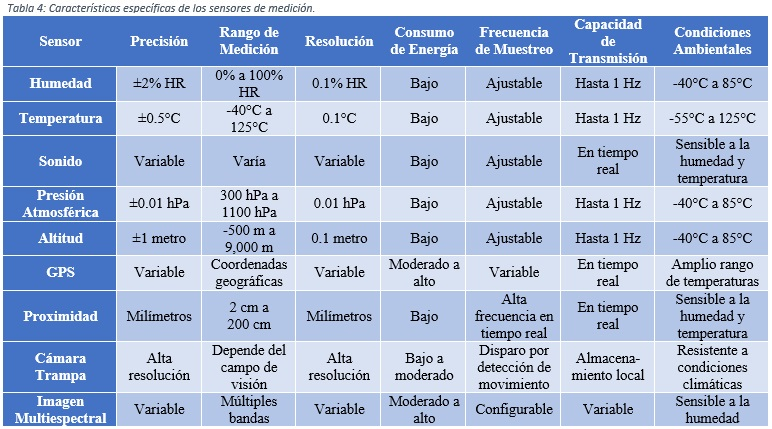
\includegraphics[width=1\linewidth, height=0.6\textheight]{imagenes/tab4_caract_sensores.jpg}
%    \label{fig:enter-label}
%\end{figure}
\newpage

% Please add the following required packages to your document preamble:
% \usepackage{multirow}
% \usepackage{longtable}
% Note: It may be necessary to compile the document several times to get a multi-page table to line up properly
% Please add the following required packages to your document preamble:
% \usepackage{multirow}
% \usepackage{graphicx}
% Please add the following required packages to your document preamble:
% \usepackage{multirow}
% \usepackage{graphicx}
\begin{table}[]
\centering
\caption{Ventajas y limitaciones de los sensores de medición. }
\label{tab:tabla2}
\resizebox{\columnwidth}{!}{%
\begin{tabular}{|c|c|c|}
\hline
\textbf{Sensor} & \textbf{Ventajas} & \textbf{Limitaciones} \\ \hline
\multirow{2}{*}{\textbf{Humedad}} & - Información precisa sobre la humedad   ambiental. & - No es relevante para todas las especies. \\
 & - Sensores   económicos y de bajo consumo. & - Requiere calibración periódica. \\ \hline
\multirow{2}{*}{\textbf{Temperatura}} & - Relevante para la mayoría de las especies. & - Rango de medición insuficiente en extremos. \\
 & - Sensores   económicos y ampliamente disponibles. & - Respuesta lenta en algunos sensores. \\ \hline
\multirow{2}{*}{\textbf{Sonido}} & - Permite la detección de sonidos relacionados   con la fauna. & - Identificación precisa desafiante. \\
 & - Útil para   monitorear actividad e interacción. & - Mayor procesamiento de datos requerido. \\ \hline
\multirow{2}{*}{\textbf{Presión Atmosférica}} & - Estimación de altitud y presión atmosférica. & - No proporciona información específica sobre   especies. \\
 & -   Proporciona información útil sobre cambios climáticos. & - Requiere calibración periódica. \\ \hline
\multirow{2}{*}{\textbf{Altitud}} & - Importante para   especies  con comportamiento altitudinal. & - No relevante para todas las especies o   hábitats. \\
 & - Responde   a cambios rápidos. & - Requiere sensores adicionales para precisión. \\ \hline
\multirow{2}{*}{\textbf{GPS}} & - Datos de ubicación precisos. & - Consumo de energía moderado. \\
 & -   Geolocalización esencial. & - Necesita visión directa con satélites. \\ \hline
\multirow{2}{*}{\textbf{Proximidad}} & - Detecta la cercanía de objetos o animales. & - Alcance limitado requiere disposición   cuidadosa. \\
 & - Bajo   consumo de energía. & - No proporciona datos detallados sobre   especies. \\ \hline
\multirow{2}{*}{\textbf{Cámara Trampa}} & - Captura imágenes de forma discreta. & - Almacenamiento y procesamiento de imágenes. \\
 & - Útil para   identificación visual de especies. & - Vulnerable a condiciones de luz y clima. \\ \hline
\multirow{2}{*}{\textbf{Imagen Multiespectral}} & - Permite análisis detallado de la vegetación y   el terreno. & - Costosa y requiere sensores específicos. \\
 & - Útil para   estudios ecológicos y agrícolas. & - No es adecuado para la detección directa de   animales. \\ \hline
\end{tabular}%
}
\end{table}

\newpage



\noindent A continuación, se presentan opciones de sensores para los tipos de mediciones mencionadas anteriormente, junto con algunas características relevantes que las diferencian entre sí.

\begin{enumerate}
    \item Humedad:
    \begin{itemize}
        \item Sensor de Humedad Capacitivo (DHT22) \cite{84}:
        \begin{enumerate}
            \item Precisión en la medición.
\item Rango de medición: 0-100\% de humedad relativa.
\item Alta estabilidad en la medición a lo largo del tiempo.
\item Costo: Aproximadamente \$5-10 USD.
\item Tamaño: Alrededor de 4 cm.
\item Peso: 3 gramos.
\item Consumo de energía: 1-1.5 mA a 3-5 volts.

        \end{enumerate}
        \item Sensor de Humedad Resistivo (HR202) \cite{85}:
        \begin{enumerate}
            \item Adecuado para aplicaciones de bajo costo.
\item Rango de medición: 0-100\% de humedad relativa.
\item Buena resistencia ante la contaminación.
\item Costo: Aproximadamente \$2-5 USD.
\item Tamaño: Cerca de 2 cm.
\item Peso: 1 gramo.
\item Consumo de energía: 0.2-0.5 mA a 3-5 volts.
\end{enumerate}
\end{itemize}

\item Temperatura
\begin{itemize}
    \item Termistor (LM35) \cite{86}:
\begin{enumerate}
        \item Alta precisión.
        \item Rango de medición: -55°C a 150°C.
        \item Respuesta rápida a cambios de temperatura.
        \item Costo: Alrededor de \$1-3 USD.
        \item Tamaño: Cerca de 1 cm.
        \item Peso: 0.1 gramos.
        \item Consumo de energía: 50-60 µA a 5 volts.
\end{enumerate}
    \item Sensor de Temperatura de Platino (PT100) \cite{87}:
\begin{enumerate}
        \item Muy alta precisión.
        \item Amplio rango de medición: -200°C a 850°C.
        \item Robusto y duradero.
        \item Costo: Aproximadamente \$20-30 USD.
        \item Tamaño: Alrededor de 5 cm.
        \item Peso: 5 gramos.
        \item Consumo de energía: Depende del circuito de interfaz, generalmente bajo.

\end{enumerate}
\end{itemize}

\item Sonido:
\begin{itemize}
    \item Micrófono de Condensador Electret (MAX4466) \cite{88}:
\begin{enumerate}
        \item Sensibilidad en la detección de sonidos.
        \item Amplio rango de frecuencia.
        \item Bajo nivel de ruido en la señal.
        \item Costo: Aproximadamente \$5-10 USD.
        \item Tamaño: Alrededor de 1.5 cm.
        \item Peso: 1 gramo.
        \item Consumo de energía: 0.5-1 mA a 3-10 volts.
\end{enumerate}
    \item Sensor de Sonido de Efecto Piezoeléctrico (KY-038) \cite{89}:
\begin{enumerate}
        \item Buena respuesta a sonidos de alta frecuencia.
        \item Amplio rango de frecuencia.
        \item Alta sensibilidad.
        \item Costo: Aproximadamente \$2-5 USD.
        \item Tamaño: Cerca de 2 cm.
        \item Peso: 1 gramo.
        \item Consumo de energía: 0.5-1 mA a 3-5 volts.

\end{enumerate}
\end{itemize}

\item Presión Atmosférica:
\begin{itemize}
    \item Sensor de Presión Piezoeléctrico (MPX5700AP) \cite{90}:
\begin{enumerate}
        \item Respuesta rápida a cambios de presión.
        \item Rango de medición: 0-10 bar.
        \item Robusto y duradero en entornos hostiles.
        \item Costo: Aproximadamente \$15-20 USD.
        \item Tamaño: Alrededor de 3 cm.
        \item Peso: 2 gramos.
        \item Consumo de energía: 1-10 mA a 3-5 volts.
\end{enumerate}
    \item Sensor de Presión Capacitivo (MS5611) \cite{91}:
\begin{enumerate}
        \item Alta precisión en la medición.
        \item Rango de medición: 10 mbar a 1200 mbar.
        \item Bajo consumo de energía para aplicaciones portátiles.
        \item Costo: Aproximadamente \$20-30 USD.
        \item Tamaño: Cerca de 2 cm.
        \item Peso: 1.5 gramos.
        \item Consumo de energía: 0.6 mA a 1.2 mA a 3-5 volts.

\end{enumerate}
\end{itemize}

\item Altitud:
\begin{itemize}
    \item Sensor de Altitud Barométrico (BMP180) \cite{92}:
\begin{enumerate}
        \item Mide altitud basada en la presión atmosférica.
        \item Precisión adecuada para aplicaciones de navegación.
        \item Bajo consumo de energía.
        \item Costo: Aproximadamente \$5-10 USD.
        \item Tamaño: Alrededor de 1.5 cm.
        \item Peso: 1 gramo.
        \item Consumo de energía: 0.5-3 mA a 1.8-3.6 volts.
\end{enumerate}
    \item Sensor de Ultrasonidos (HC-SR04) \cite{93}:
\begin{enumerate}
        \item Mide la distancia desde el sensor al objeto mediante ultrasonidos.
        \item Amplio rango de detección.
        \item Alta velocidad de respuesta en la medición.
        \item Costo: Aproximadamente \$2-5 USD.
        \item Tamaño: Cerca de 4 cm.
        \item Peso: 3 gramos.
        \item Consumo de energía: 2 mA a 5 volts.

\end{enumerate}
\end{itemize}

\item GPS:
\begin{itemize}
    \item Módulo GPS de un solo canal (NEO-6M) \cite{94}:
\begin{enumerate}
        \item Precisión estándar en geolocalización.
        \item Bajo consumo de energía.
        \item Pequeño y liviano, ideal para dispositivos compactos.
        \item Costo: Aproximadamente \$10-20 USD.
        \item Tamaño: Alrededor de 4 cm.
        \item Peso: 10 gramos.
        \item Consumo de energía: 30-40 mA a 3-5 volts.
\end{enumerate}
    \item Módulo GPS de varios canales (u-blox NEO-M8N) \cite{95}:
\begin{enumerate}
        \item Mayor precisión y capacidad de adquisición rápida de señales GPS.
        \item Soporte para múltiples sistemas de navegación, como GPS, GLONASS y Galileo.
        \item Alta velocidad de actualización.
        \item Costo: Aproximadamente \$20-30 USD.
        \item Tamaño: Cerca de 5 cm.
        \item Peso: 15 gramos.
        \item Consumo de energía: 30-40 mA a 3-5 volts.

\end{enumerate}
\end{itemize}

\item Proximidad:
\begin{itemize}
    \item Sensor de Infrarrojos de Reflexión (TCRT5000) \cite{96}:
\begin{enumerate}
        \item Detecta objetos cercanos por reflexión de luz infrarroja.
        \item Alta velocidad de respuesta en la detección.
        \item Costo: Aproximadamente \$1-5 USD.
        \item Tamaño: Cerca de 1 cm.
        \item Peso: 2 gramos.
        \item Consumo de energía: 1-5 mA a 3-5 volts.
\end{enumerate}
    \item Sensor Ultrasónico de Proximidad (HC-SR04) \cite{97}:
\begin{enumerate}
        \item Mide la distancia entre el sensor y el objeto mediante ultrasonidos.
        \item Amplio rango de detección y bajo costo.
        \item Alta sensibilidad.
        \item Costo: Aproximadamente \$1-5 USD.
        \item Tamaño: Alrededor de 4 cm.
        \item Peso: 3 gramos.
        \item Consumo de energía: 15 mA a 5 volts.

\end{enumerate}
\end{itemize}

\item Cámara Trampa:
\begin{itemize}
    \item Cámara de Infrarrojos (Browning Strike Force) \cite{98}:
\begin{enumerate}
        \item Captura imágenes en condiciones de poca luz.
        \item Función de visión nocturna por infrarrojos para imágenes nítidas en la oscuridad.
        \item Alta velocidad de disparo para capturar acciones rápidas.
        \item Costo: Aproximadamente \$150-200 USD.
        \item Tamaño: Alrededor de 12 cm x 8 cm.
        \item Peso: 160 gramos.
        \item Consumo de energía: Variable, en modo de espera consume muy poca energía.
\end{enumerate}
    \item Cámara de Alta Resolución (PR700) \cite{99}:
\begin{enumerate}
        \item Captura imágenes detalladas de alta calidad.
        \item Diseñada para resistir condiciones climáticas adversas en entornos de monitoreo de vida silvestre.
        \item Amplio rango de temperatura de funcionamiento.
        \item Costo: Aproximadamente \$500-800 USD.
        \item Tamaño: Cerca de 15 cm x 8 cm.
        \item Peso: 400 gramos.
        \item Consumo de energía: Variable, pero bajo en modo de espera.

\end{enumerate}
\end{itemize}

\item Imagen Multiespectral:
\begin{itemize}
    \item Cámara Multiespectral de Detección Remota (Parrot Sequoia) \cite{100}:
\begin{enumerate}
        \item Captura información en múltiples bandas espectrales.
        \item Permite la generación de índices vegetativos de alta precisión.
        \item Ligera y fácil de montar en drones.
        \item Costo: Aproximadamente \$3,000-4,000 USD.
        \item Tamaño: Alrededor de 10 cm x 6 cm.
        \item Peso: 110 gramos.
        \item Consumo de energía: 8 W.
\end{enumerate}
    \item Cámara Multiespectral Hiperespectral (Headwall Nano-Hyperspec) \cite{101}:
\begin{enumerate}
        \item Captura información en una amplia gama de bandas espectrales.
        \item Mayor capacidad para la detección de diferencias sutiles en la reflectancia espectral de los objetos
        \item Utilizada en aplicaciones de investigación científica avanzada.
        \item Costo: Varía según las especificaciones, generalmente en el rango de \$10,000-30,000 USD.
        \item Tamaño: Varía entre 10 cm x 10 cm a 20 cm x 20 cm , según la configuración.
        \item Peso: Varía entre 200 gramos a 1 kilogramo, según la configuración.
        \item Consumo de energía: Varía según la configuración, típicamente más alto que otros sensores.
\end{enumerate}

\end{itemize}
\end{enumerate}
    
\subsection{Selección de los Sensores}
La selección de sensores desempeña un papel fundamental en el diseño de nuestro sistema de monitoreo. Cada sensor cumple un papel específico en la recopilación de datos críticos para el éxito de este proyecto. Por lo que se ha optado por medir la temperatura, utilizar un módulo GPS y la captura de imagen con una cámara trampa. A continuación, se justifica esta selección:

 \begin{itemize}
     \item \textbf{Medición de la Temperatura (seleccionando Termistor LM35):}

La temperatura es un factor ambiental crítico que puede afectar la distribución y el comportamiento de las especies. Los cambios en la temperatura pueden tener un impacto directo en la actividad de los animales, su reproducción y su búsqueda de alimento. Monitorear la temperatura es esencial para comprender cómo los cambios climáticos pueden estar afectando a las especies en peligro de extinción.

El termistor LM35 es una elección adecuada para medir la temperatura debido a su alta precisión, su amplio rango de medición y su facilidad de integración. Además, su bajo consumo de energía lo hace adecuado para ser situado en lugares remotos \cite{86}. En la \hyperref[termistor]{Figura \ref{termistor}} se puede ver un ejemplo del termistor LM35.
\begin{figure}[H]
  \centering
  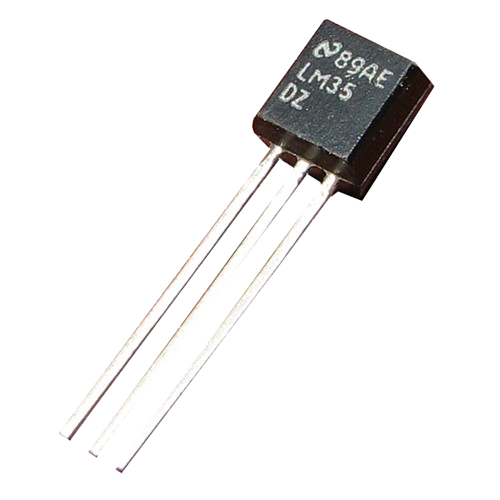
\includegraphics[width=0.4\textwidth]{imagenes/termistor.png}
  \caption{Termistor LM35.}
  \label{termistor}
\end{figure}

\item \textbf{Geolocalización (seleccionando Módulo GPS Neo-6M):}

La capacidad de rastrear y registrar con precisión la ubicación geográfica de las observaciones es fundamental en proyectos de monitoreo de especies. Ayuda a determinar la distribución espacial de las especies, sus patrones de migración y su relación con el hábitat.

El módulo GPS Neo-6M es elegido debido a su precisión y su capacidad para rastrear múltiples satélites de diferentes sistemas de navegación, lo que mejora la precisión de la geolocalización. Su bajo consumo de energía lo hace adecuado para drones \cite{94}. En la \hyperref[gps]{Figura \ref{gps}} se puede ver un ejemplo del módulo GPS Neo-6M.
\begin{figure}[H]
  \centering
  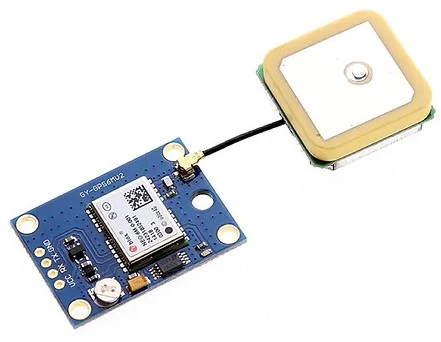
\includegraphics[width=0.4\textwidth]{imagenes/gps.jpg}
  \caption{Módulo GPS Neo-6M.}
  \label{gps}
\end{figure}

\item \textbf{Captura de Imágenes (seleccionando Cámara Trampa PR-700):}

Las imágenes visuales son una fuente invaluable de datos en proyectos de monitoreo de vida silvestre. Permiten la identificación de especies, el seguimiento de la actividad y el análisis de la salud de los individuos.

La cámara trampa PR-700 se selecciona debido a su capacidad para capturar imágenes de alta resolución y calidad en condiciones diversas, incluyendo situaciones de poca luz o nocturnas. Su resistencia a condiciones climáticas adversas y su capacidad para capturar imágenes de vida silvestre de manera discreta la hacen ideal para este proyecto \cite{99}. En la \hyperref[camara]{Figura \ref{camara}} se puede ver un ejemplo de la cámara trampa PR-700.
\begin{figure}[H]
  \centering
  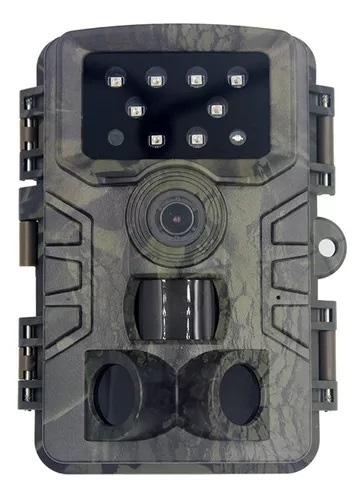
\includegraphics[width=0.4\textwidth, height=0.35 \textwidth]{imagenes/camara.jpg}
  \caption{Módulo GPS Neo-6M.}
  \label{camara}
\end{figure}

 
 \end{itemize}

\noindent La elección de medir la temperatura, utilizar un módulo GPS y una cámara trampa se basa en la relevancia de estas mediciones para el propósito de este proyecto. El termistor LM35 proporcionará datos precisos sobre las condiciones ambientales que pueden influir en el comportamiento de las especies, mientras que el módulo GPS Neo-6M permitirá geolocalizar con exactitud nuestras observaciones y rastrear los movimientos de las especies. Por último, la cámara trampa PR-700 brindará imágenes de alta calidad que serán esenciales para la identificación y el análisis de las especies.\\
Esta elección de sensores se basa en un análisis detallado de diversos factores, entre los cuales se destaca la consideración de costos, tamaño, peso y consumo energético. En primer lugar, el costo de los sensores es un factor muy importante en este proyecto, por lo que se han seleccionado sensores que ofrecen una excelente relación calidad-precio, permitiendo mantener el proyecto dentro de un presupuesto razonable y alcanzable.\\
En cuanto al tamaño y el peso, es esencial que los sensores sean compactos y livianos para ser instalados sin dificultad en las ubicaciones terrestres identificadas, como árboles o estructuras diseñadas para este propósito.\\
Además, la eficiencia energética sigue siendo esencial, ya que estos sensores deberán funcionar de manera autónoma durante períodos prolongados. Los sensores seleccionados son conocidos por su eficiencia energética, lo que minimiza el drenaje de la batería y garantiza un tiempo de operación adecuado. Esto es esencial para recopilar datos de monitoreo durante períodos prolongados sin requerir frecuentes cambios de batería o recarga.\\
Concluyendo en que los sensores seleccionados no sólo son relevantes desde el punto de vista técnico, sino que también se ajustan de manera óptima a los aspectos económicos, logísticos y operativos del proyecto de monitoreo de especies en peligro de extinción.

\newpage
\section{Análisis de la WSN (Red Inalámbrica de Sensores)}

El diseño y la operación de la red inalámbrica de sensores (WSN) debe estar meticulosamente planificado para garantizar la recopilación precisa de datos en tiempo real. Por lo que hay que examinar detenidamente los aspectos clave de la WSN que se piensan implementar en este proyecto, destacando sus características técnicas y consideraciones críticas.
\subsection{Arquitectura de la WSN:}
Existen dos arquitecturas principales para la implementación de redes inalámbrica de sensores: la arquitectura cliente-servidor y la arquitectura peer-to-peer (P2P). Las cuales se describen en la \hyperref[tablaarqui]{Tabla \ref{tablaarqui}: Comparación entre Arquitectura Cliente-Servidor y Peer-to-Peer (P2P).}


Se selecciona la arquitectura Cliente-Servidor para la WSN debido a la necesidad de una gestión centralizada que permita un control preciso de la red y optimice el procesamiento de datos. Dada la importancia de coordinar eficientemente las operaciones de monitoreo, así como de gestionar y distribuir recursos de manera controlada, la arquitectura Cliente-Servidor ofrece un marco robusto para lograr estos objetivos. Además, la posibilidad de realizar mantenimiento y actualizaciones de manera remota resulta crucial para asegurar un funcionamiento continuo y adaptativo de la red. La arquitectura Cliente-Servidor proporciona una estructura organizativa sólida que se alinea con los requisitos específicos del monitoreo a realizar.
\newpage
\begin{table}[H]
\centering
\caption{Comparación entre Arquitectura Cliente-Servidor y Peer-to-Peer (P2P).}
\begin{tabular}{|p{2.5cm}|p{6.5cm}|p{6.5cm}|}
\hline
\cellcolor[HTML]{C0C0C0}\textbf{Arquitectura} & \cellcolor[HTML]{C0C0C0}\textbf{Cliente-Servidor} & \cellcolor[HTML]{C0C0C0}\textbf{Peer-to-Peer (P2P)} \\
\hline
\textbf{Descripción} &
La red está organizada en torno a un nodo central denominado \textquotedbl{}servidor\textquotedbl{} y múltiples nodos periféricos llamados \textquotedbl{}clientes\textquotedbl{}. El servidor coordina y gestiona las operaciones, mientras que los clientes recopilan datos y los envían al servidor para su procesamiento \cite{clienteservidor}.
&
Todos los nodos actúan como iguales, compartiendo y procesando datos de manera descentralizada. No hay un nodo central que coordine las operaciones; en cambio, cada nodo puede comunicarse directamente con otros nodos en la red. Esta arquitectura es más distribuida y autónoma\cite{p2p}.
\\
\hline
\textbf{Ventajas} &
-Gestión de Recursos: Permite una gestión eficaz de recursos, ya que el servidor puede asignar tareas y controlar el flujo de datos.
&
-Descentralización: Elimina la dependencia de un servidor central, mejorando la redundancia y robustez de la red.
\\
&
-Control Centralizado: Facilita la administración y coordinación eficientes de la red.
&
-Escalabilidad: Puede ser más escalable, ya que la adición de nuevos nodos no requiere cambios significativos en la infraestructura existente.
\\
&
-Mantenimiento Remoto: Facilita actualizaciones y mantenimiento remotos.
&
\\
\hline
\textbf{Desventajas} &
-Dependencia del Servidor: Si el servidor falla, la red puede volverse inoperable.
&
-Coordinación Desafiante: La coordinación y gestión pueden ser desafiantes debido a la falta de un punto centralizado de control.
\\
&
-Posible Cuello de Botella: El servidor puede convertirse en un cuello de botella.
&
-Problemas de Seguridad: La seguridad puede ser más compleja de implementar en una red P2P debido a la naturaleza distribuida de la arquitectura.
\\
\hline
\end{tabular}
\label{tablaarqui}
\end{table}


\subsection{Topología de la WSN}
La topología de la red inalámbrica de sensores se organizará de manera que garantice una cobertura eficiente de la zona de monitoreo. Se evaluarán opciones como topología en malla, árbol o estrella, ya que cada una ofrece enfoques distintos para gestionar la conectividad entre los nodos de la red, como se puede ver a continuación:
\begin{itemize}
\item \textbf{Topología en Malla:} En esta topología, cada nodo de la red se conecta con múltiples nodos vecinos, formando una estructura de malla interconectada. Esto crea múltiples rutas de comunicación entre los nodos, aumentando la redundancia y la fiabilidad de la red. Si un nodo falla o se desconecta, la red puede encontrar una ruta alternativa para mantener la comunicación \cite{malla}. Usualmente se utiliza en aplicaciones donde la redundancia y la tolerancia a fallos son críticas, como en entornos industriales o militares.\\
Ventaja: Redundancia y tolerancia a fallos. La presencia de múltiples rutas de comunicación permite que la red se adapte a fallos individuales sin perder conectividad. Ideal para entornos críticos donde la fiabilidad es esencial.\\
Desventaja: Mayor complejidad de gestión y configuración. La necesidad de gestionar varias conexiones y rutas puede aumentar la complejidad del diseño y la administración de la red.
\item \textbf{Topología en Árbol:} En este tipo de  topología, los nodos se organizan jerárquicamente, con un nodo central (raíz) que se comunica con nodos secundarios, y estos, a su vez, pueden tener nodos hijos adicionales. La comunicación sigue una estructura descendente desde la raíz hasta los nodos periféricos \cite{arbol}. Usualmente se utiliza en aplicaciones donde hay un nodo central de control y los nodos periféricos recopilan datos, como en sistemas de monitorización de edificios.\\
Ventaja: Jerarquía y escalabilidad. La estructura jerárquica facilita la gestión y permite escalar la red añadiendo más nodos periféricos. Es eficiente para aplicaciones que requieren una estructura de control centralizado.\\
Desventaja: Vulnerabilidad ante la falla del nodo central. Si el nodo raíz falla, toda la rama de la red podría perder conectividad, lo que podría ser problemático en situaciones críticas.
\item \textbf{Topología en Estrella:} En esta topología, todos los nodos de la red se conectan directamente a un nodo central (hub o coordinador), pero no se conectan entre sí. Todas las comunicaciones pasan a través del nodo central. Esto simplifica la gestión y la configuración de la red \cite{estrella}. Usualmente se utiliza en aplicaciones donde la simplicidad, la facilidad de configuración y el bajo consumo energético es prioritario, como en sistemas de monitoreo y control remoto.\\
Ventaja: Sencillez y facilidad de gestión. La conexión directa de todos los nodos al centro simplifica la gestión y la configuración. Es fácil de entender y mantener.\\
Desventaja: Vulnerabilidad del nodo central. Si el nodo central (hub) falla, todos los nodos quedan desconectados. Puede ser menos apropiada en aplicaciones críticas que requieren alta disponibilidad.
\end{itemize}
Se elige una topología en estrella para la WSN por su facilidad de implementación, gestión centralizada y capacidad para identificar rápidamente problemas. La sencillez en la instalación y configuración de los sensores permite una rápida implementación en el terreno, mientras que la estructura en estrella facilita la administración centralizada desde un nodo principal, optimizando la eficiencia operativa. Además, la rápida identificación de problemas individuales sin afectar a otros nodos simplifica el mantenimiento y garantiza una operación continua. Aunque se reconoce la vulnerabilidad potencial del nodo central, medidas de seguridad y redundancia pueden mitigar este riesgo, respaldando así la elección de la topología en estrella para el monitoreo efectivo de especies en peligro de extinción.

\subsection{Microprocesador de la WSN}
En la selección del microprocesador para la WSN y para los collares de los animales, se evaluaron diversas opciones considerando factores clave como consumo energético, capacidad de procesamiento y facilidad de integración, como se muestra a continuación:
\begin{itemize}
\item \textbf{Arduino Pro Micro:} Es  una placa de desarrollo basada en el microcontrolador ATmega32U4. Destaca por su tamaño compacto y bajo consumo de energía, haciéndolo ideal para dispositivos portátiles y con restricciones de energía. Aunque tiene menos capacidad de procesamiento que algunas alternativas, es suficiente para aplicaciones específicas y cuenta con una comunidad activa de desarrolladores que brindan soporte y una amplia gama de bibliotecas \cite{arduino}.
\item \textbf{Raspberry Pi Zero W:} Es una mini computadora de bajo costo con conectividad inalámbrica. Aunque es más potente que Arduino Pro Micro y puede ejecutar un sistema operativo completo, tiene un consumo de energía relativamente mayor. Su versatilidad lo hace adecuado para proyectos más complejos que requieren un sistema operativo, pero puede ser excesivo para dispositivos pequeños y de bajo consumo \cite{pizero}. 
\item \textbf{ESP32:} Es un microcontrolador de bajo costo y bajo consumo de energía con conectividad Wi-Fi y Bluetooth. Ofrece un equilibrio entre capacidad de procesamiento y eficiencia energética, lo que lo hace atractivo para diversas aplicaciones \cite{esp32}. Sin embargo, su tamaño y complejidad pueden no ser ideales para dispositivos extremadamente pequeños como collares de monitoreo.
\end{itemize}
La elección de Arduino Pro Micro para la WSN y los collares se fundamenta en su bajo consumo energético, capacidad suficiente para tareas específicas de monitoreo, y su tamaño compacto. Estas características son esenciales para garantizar una operación de larga duración de los collares, mientras que la simplicidad y confiabilidad hacen de Arduino Pro Micro una opción óptima para la WSN, donde la eficiencia y la estabilidad son prioritarias. La consistencia en la elección de Arduino Pro Micro simplifica el desarrollo, la programación y el mantenimiento de la red de monitoreo.

\subsection{Fuente de Energía de la WSN}
La elección de la fuente de energía para el microprocesador de la WSN es un aspecto crítico en el diseño de dispositivos de monitoreo, ya que afecta directamente la autonomía y la eficiencia operativa. Entre las opciones comunes se encuentran las baterías recargables de iones de litio (Li-Ion) y las baterías alcalinas.
\begin{itemize}
\item \textbf{Baterías Recargables de Iones de Litio (Li-Ion):} Estas baterías son conocidas por su alta densidad de energía y su capacidad de ser recargadas, lo que las hace ideales para dispositivos de larga duración. Ofrecen una tensión constante y tienen una vida útil prolongada. Sin embargo, suelen ser más costosas y requieren circuitos de protección para evitar sobrecargas o descargas excesivas \cite{litio}.
\item \textbf{Baterías Alcalinas:} Las baterías alcalinas son una opción tradicional y fácilmente disponibles en el mercado. Aunque son más económicas, su vida útil es limitada, y una vez agotadas, deben ser reemplazadas. También pueden experimentar caídas de voltaje a medida que se descargan, lo que podría afectar el rendimiento del microprocesador \cite{alcalinas}.
\end{itemize}
La elección de baterías recargables de iones de litio se fundamenta en la necesidad de una fuente de energía eficiente y de larga duración. Para dispositivos de monitoreo que requieren una autonomía prolongada, las baterías Li-Ion ofrecen una solución confiable. Aunque su costo inicial puede ser superior, su capacidad de recarga y su vida útil más extensa reducen los costos a largo plazo y minimizan la necesidad de reemplazo frecuente. Además, los circuitos de protección pueden integrarse para garantizar un uso seguro y optimizar la eficiencia de la batería durante la operación continua del microprocesador.

\subsection{Comunicación Inalámbrica de la WSN}
La eficacia de la comunicación inalámbrica es esencial para el éxito de nuestro sistema de monitoreo, ya que se debe permitir la transferencia archivos de datos, así como de archivos multimedia. Por lo que se consideran las siguientes opciones:
\begin{itemize}
\item \textbf{LoRa UART 868/915 MHz:} LoRa (Long Range) en la banda de frecuencia UART 868/915 MHz es una elección ideal para la transmisión de archivos de texto en entornos donde se requiere un alcance extenso y una baja tasa de transferencia de datos. Su capacidad para penetrar obstáculos y brindar una conectividad confiable a larga distancia lo hace adecuado para la comunicación eficiente de datos de texto entre los nodos de la red. La baja demanda de energía de LoRa contribuye a la eficiencia operativa, crucial para prolongar la duración de la batería de los dispositivos de monitoreo \cite{lora}.
\item \textbf{Antenas WiFi:}
Las antenas WiFi son una elección apropiada cuando se busca una transmisión rápida y eficiente de archivos de video. La tecnología WiFi ofrece un ancho de banda significativamente mayor en comparación con LoRa, permitiendo la transmisión de datos de video con calidad adecuada. Aunque su alcance puede ser más limitado en comparación con LoRa, la prioridad aquí es la velocidad de transmisión para garantizar la entrega oportuna de archivos de video desde los drones a la estación base. El uso de antenas WiFi se justifica por su capacidad para manejar el alto volumen de datos asociado con la transmisión de video en tiempo real \cite{119}.
\item \textbf{Bluetooth:} Es una tecnología inalámbrica adecuada para la comunicación a corta distancia. Aunque su alcance es más limitado en comparación con LoRa, es ideal para la comunicación entre dispositivos cercanos, como la interacción entre drones y sensores terrestres en un entorno localizado. Su baja demanda de energía también lo hace adecuado para aplicaciones de corto alcance \cite{bluetooth}.
\item \textbf{RFID (Identificación por Radiofrecuencia):} Es una tecnología que se utiliza para la identificación sin contacto a corta distancia. Puede ser útil para el seguimiento y la identificación de individuos o elementos específicos en un área cercana. Sin embargo, su aplicación se limita a distancias cortas y a la identificación más que a la transmisión de datos sustanciales \cite{rfid}.
\end{itemize}
Se selecciona LoRa UART 868/915 MHz para la transmisión de archivos de texto entre los collares gps y la WSN, así como entre la WSN y los drones, debido a su capacidad única para proporcionar una conectividad confiable a larga distancia con un bajo consumo de energía. Dada la naturaleza extensa del área de monitoreo y la necesidad de establecer una red robusta entre los nodos de drones y WSN, LoRa se destaca por su excepcional alcance y capacidad para penetrar obstáculos, garantizando una comunicación estable incluso en entornos desafiantes. Su baja tasa de transferencia de datos es adecuada para la transmisión de archivos de texto críticos para el monitoreo de especies en peligro de extinción, contribuyendo así a la eficiencia operativa y a la duración de la batería.\\
Por otra parte, se selecciona la antena WiFi para la transmisión de archivos de video por la necesidad de un ancho de banda significativo y una velocidad de transmisión rápida. Aunque su alcance puede ser más limitado en comparación con LoRa, la prioridad aquí es la velocidad y calidad de transmisión para garantizar la entrega oportuna de archivos de video. La capacidad de las antenas WiFi para manejar grandes volúmenes de datos los hace esenciales para la recopilación eficiente de información visual en el contexto del monitoreo de especies.
\subsection{Módulo de Almacenamiento de la WSN}
Existen diversas opciones de módulos de almacenamiento para integrar en nuestra red inalámbrica de sensores (WSN). Entre ellas, consideramos módulos USB y módulo MicroSD, como se puede observar a continuación:
\begin{itemize}
\item \textbf{Módulos USB:} Los módulos USB para almacenamiento ofrecen una solución conveniente para la transferencia y almacenamiento de datos. Estos dispositivos suelen ser compactos y fáciles de usar, conectándose directamente a los puertos USB de los dispositivos compatibles. Además, muchos de ellos admiten una variedad de formatos de tarjetas de memoria y unidades USB \cite{usb}.\\
Ventajas:	
\begin{itemize}[label=o]
\item \textbf{Portabilidad:} Los módulos USB son pequeños y ligeros, lo que facilita su transporte y conexión a diferentes dispositivos.
\item \textbf{Interfaz estándar:} La interfaz USB es universal, lo que garantiza la compatibilidad con una amplia gama de dispositivos.
\item \textbf{Capacidades variables:} Disponibles en diversas capacidades de almacenamiento para adaptarse a las necesidades específicas.
\end{itemize}
Desventajas:
\begin{itemize}[label=o]
\item \textbf{Mayor consumo de energía:} Algunos módulos USB pueden consumir más energía en comparación con otras soluciones, lo que puede ser relevante en aplicaciones con restricciones energéticas.
\item \textbf{Exposición física:} Al estar conectados externamente, los módulos USB pueden estar expuestos a condiciones climáticas adversas y riesgos físicos.
\end{itemize}

\item \textbf{Adaptadores de tarjetas MicroSD:} Estos adaptadores permiten la conexión de tarjetas de memoria MicroSD a dispositivos que no tienen un puerto MicroSD integrado. Suelen ser simples y compactos, proporcionando una interfaz eficiente entre la tarjeta de memoria y el dispositivo anfitrión \cite{122}.
Ventajas:
\begin{itemize}[label=o]
\item \textbf{Tamaño compacto:} Los adaptadores MicroSD son pequeños y livianos, ocupando poco espacio y siendo fáciles de integrar en dispositivos.
\item \textbf{Compatibilidad:} Al admitir tarjetas MicroSD estándar, ofrecen una gran flexibilidad y variedad de opciones de almacenamiento.
\item \textbf{Bajo consumo energético:} Consumen menos energía en comparación con algunas soluciones USB.
\end{itemize}
Desventaja:
\begin{itemize}[label=o]
\item \textbf{
Manipulación Sensible:} Dada su naturaleza pequeña, los adaptadores de tarjetas MicroSD pueden ser delicados y requerir manejo cuidadoso.
\end{itemize}
\end{itemize}
El módulo MicroSD Card Adapter (modelo MLMSD) destaca por su compatibilidad con tarjetas MicroSD, que ofrecen capacidades de almacenamiento significativas y una amplia disponibilidad en el mercado. La elección de este adaptador se basa en su simplicidad, bajo consumo de energía y facilidad de integración con microcontroladores, como el Arduino Pro Micro que cuentan collares y la WSN. Además, la tecnología MicroSD proporciona un acceso rápido y eficiente a los datos almacenados, permitiendo una gestión ágil y local de la información recopilada por los sensores distribuidos en el terreno de monitoreo. Con esta elección, aseguramos un sistema de almacenamiento robusto y confiable que se alinea perfectamente con los requisitos operativos de nuestra WSN.
La elección de este módulo implica la implementación de memorias MicroSD como solución de almacenamiento para los archivos de datos generados tanto por el microprocesador en los collares y en la WSN, como por los archivos de video las cámaras trampa.

%%%%%%%%%%%%%%%%%%%%%%%%%%%%%%%%%%%%
\newpage
\section{Análisis de los Drones.}
El empleo de drones en este proyecto presenta varias ventajas significativas que justifican su elección como plataforma para la recolección de datos. A continuación, se detallan las razones clave:
\begin{enumerate}
  \item \textbf{Acceso a Áreas Remotas y de Difícil Acceso:} Los drones permiten llegar a áreas remotas y de difícil acceso para los humanos. Esto es crucial en estudios de biología de campo, donde algunas especies habitan en entornos inexplorados o de difícil acceso terrestre.
  \item \textbf{Reducción del Impacto Ambiental:} La presencia humana en áreas naturales puede perturbar a las especies y afectar negativamente a los hábitats frágiles. Los drones reducen este impacto al volar a altitudes que minimizan la interferencia con la vida silvestre y al evitar la alteración de la vegetación.
  \item \textbf{Eficiencia en la Recolección de Datos:} Los enjambres de drones pueden cubrir grandes áreas en poco tiempo y recolectar datos simultáneamente, mejorando significativamente la eficiencia en la recolección de datos en comparación con métodos tradicionales de campo.
  \item \textbf{Menor Riesgo para los Investigadores:} Al utilizar drones, se reducen los riesgos asociados con largos y agotadores recorridos a pie en terrenos complicados, mejorando la seguridad de los investigadores y permitiendo la exploración de áreas potencialmente peligrosas.
  \item \textbf{Programación de Rutas Precisas:} Los drones pueden ser programados para seguir rutas preestablecidas, garantizando una cobertura completa de las áreas de interés, lo cual es valioso en estudios de biología de campo donde la precisión en la recolección de datos es fundamental.
\end{enumerate}

\subsection{Tipo de Dron}

Como se pudo ver en la sección\hyperref[marcodrones]{8.3 Enjambre de drones} del Marco Teórico de este documento, existen varios tipos de drones, como cuadricópteros, hexacópteros, etc. Por lo que para seleccionar el tipo de dron a utilizar en este proyecto, se realizará un análisis comparativo considerando diferentes aspectos.
\begin{itemize}
    \item \textbf{Tamaño:}
Al analizar las categorías de tamaño de drones, que abarcan desde nano hasta grande, cada clasificación presenta ventajas y limitaciones particulares. \\
Los drones de tamaño nano y micro son extremadamente compactos y ligeros, ideales para maniobras precisas y operaciones en espacios reducidos. Sin embargo, su capacidad de carga, autonomía y estabilidad en condiciones climáticas adversas pueden ser limitadas.\\
En el otro extremo, los drones de tamaño grande, con una envergadura superior a 2 metros, ofrecen una mayor capacidad de carga y resistencia a condiciones climáticas desafiantes. Sin embargo, suelen ser más costosos, difíciles de transportar y pueden requerir infraestructuras especializadas para su despliegue \cite{tipostamanios}.\\
Por lo que se considera más adecuado el tamaño medio, que abarca desde 500 mm hasta 2 metros, esto se justifica considerando un equilibrio entre las ventajas de las categorías más pequeñas y grandes. Los drones de tamaño medio ofrecen una combinación óptima de capacidad de carga, autonomía y estabilidad. Presentan la versatilidad necesaria para adaptarse a diferentes entornos de monitoreo, desde áreas densamente arboladas hasta terrenos abiertos, sin comprometer significativamente la maniobrabilidad.\\
Además, los drones de tamaño medio son más fáciles de transportar y desplegar en comparación con sus contrapartes más grandes, lo que facilita su movilidad entre ubicaciones de monitoreo. Esta característica es esencial en escenarios de campo donde la accesibilidad y la rapidez en la implementación del monitoreo son factores críticos.

\item \textbf{Peso máximo al despegue (MTOW):}
La categoría de peso máximo al despegue (MTOW) de los drones, que varía desde menos de 0.5 kg hasta más de 25 kg, presenta consideraciones críticas en términos de capacidad de carga, autonomía y restricciones regulatorias. Cada rango de peso tiene implicaciones específicas para el monitoreo de especies en peligro de extinción.\\
En la categoría de menos de 0.5 kg, los drones son ligeros y compactos, lo que facilita la portabilidad y el despliegue rápido. Sin embargo, su capacidad de carga es limitada, lo que podría restringir la instalación de sensores avanzados y dispositivos de recolección de datos más robustos. Además, pueden verse afectados por condiciones climáticas adversas debido a su menor estabilidad.\\
En la categoría de 0.5–5 kg, los drones ofrecen un equilibrio crucial entre portabilidad y capacidad de carga. Este rango de peso permite la instalación de sensores especializados, cámaras de alta resolución y sistemas de telemetría más avanzados. La autonomía también tiende a ser mayor en comparación con drones más livianos, lo que es fundamental para la eficiencia operativa en misiones extensas de monitoreo.\\
En la categoría de 5–25 kg, los drones tienen una mayor capacidad de carga, lo que podría permitir la integración de equipos más pesados y potentes. Esto sería beneficioso para misiones que requieran sensores de mayor tamaño, baterías de mayor capacidad o equipos especializados. Sin embargo, la portabilidad y la agilidad podrían verse comprometidas debido al mayor tamaño y peso del dron. Además, la autonomía podría ser menor en comparación con drones más ligeros.\\
Para drones con un MTOW superior a 25 kg, se abre la posibilidad de utilizar sistemas aún más avanzados y pesados. Estos drones podrían ser ideales para aplicaciones que requieran equipos especializados de alta gama, como sensores de imagen multiespectral de mayor tamaño, sistemas de muestreo de aire o equipos científicos avanzados. No obstante, su uso puede estar sujeto a regulaciones más estrictas y requerir permisos especiales \cite{tiposdrones}.\\
La elección de drones con un MTOW de 0.5–5 kg es la más adecuada para el monitoreo de especies en peligro de extinción. Aunque los drones más pesados ofrecen capacidades avanzadas, suelen ser más adecuados para aplicaciones especializadas y pueden estar sujetos a restricciones regulatorias más estrictas. El rango de 0.5–5 kg proporciona el equilibrio adecuado entre capacidad de carga, autonomía y flexibilidad operativa, lo que resulta fundamental para abordar los desafíos específicos del monitoreo de la biodiversidad en entornos variados. Además, en términos de regulaciones, los drones de esta categoría suelen estar sujetos a menos restricciones que los de mayor MTOW, facilitando la obtención de permisos y cumplimiento normativo.

\item \textbf{Alcance (Distancia/Tipo de Operación):}
Al comparar los drones según el alcance de operación, se encuentran tres categorías clave: corto alcance (<0.5 millas), medio alcance (0.5–5 millas) y largo alcance (>5 millas). \\
Los drones de corto alcance son ideales para misiones en entornos cercanos y confinados, donde la distancia entre la estación base y el dron es relativamente corta. Estos drones son adecuados para operaciones de baja altitud y vuelos a corta distancia, pero pueden no ser eficientes en la cobertura de áreas extensas.\\
Los drones de largo alcance, por otro lado, ofrecen la capacidad de cubrir distancias significativas, pero suelen estar diseñados para aplicaciones más especializadas, como la monitorización de oleoductos o la exploración de grandes extensiones de terreno. Pero para el monitoreo de especies en peligro de extinción, donde la atención puede centrarse en áreas específicas, los drones de largo alcance pueden no ser la opción más eficiente \cite{tiposdrones}.\\
Por lo que, debido a su versatilidad en términos de cobertura de área y eficiencia operativa, los drones de medio alcance (0.5–5 millas) se consideran la mejor opción. Estos drones proporcionan un equilibrio adecuado entre la capacidad de cubrir distancias moderadas y la flexibilidad para operar en entornos diversos. Además, se alinean con las regulaciones de vuelo visual lineal (VLOS) y visual extendida (EVLOS), lo que garantiza operaciones seguras y dentro de los límites reglamentarios.

\item \textbf{Ala:}
Los drones de ala fija son eficientes para cubrir grandes áreas y realizar misiones de largo alcance. Sin embargo, suelen requerir pistas de despegue y aterrizaje, lo que limita su utilidad en áreas con acceso limitado. Estos drones son más adecuados para aplicaciones como la cartografía y la vigilancia aérea extensiva, pero pueden no ser la opción más práctica para el monitoreo detallado de especies en hábitats complejos.\\
Los drones de ala giratoria, también conocidos como multi-rotores, utilizan rotores para generar sustentación y control, lo que les proporciona una capacidad excepcional de despegue y aterrizaje vertical (VTOL). Esta característica es crucial al operar en áreas con limitaciones espaciales, como bosques densos o áreas montañosas. Los multi-rotores ofrecen una excelente maniobrabilidad, lo que facilita el vuelo a baja altitud y la captura de datos detallados en entornos complejos. Su capacidad para mantenerse estacionarios es esencial al realizar tareas de monitoreo que requieren observación precisa, como el seguimiento de especies animales \cite{tiposdrones}.\\
Los drones híbridos ofrecen una combinación de las ventajas de las alas giratorias y fijas. Pueden despegar y aterrizar verticalmente, pero también pueden cambiar a vuelo de ala fija para mayor eficiencia en distancias largas. Aunque son versátiles, la complejidad de diseño y el costo adicional pueden superar los beneficios específicos requeridos para el monitoreo de especies en peligro de extinción.\\
Es por ello que la elección de drones de ala giratoria, especialmente en la configuración multi-rotor, se justifica por su capacidad VTOL, maniobrabilidad precisa y eficiencia en la cobertura de áreas diversas, características esenciales para el monitoreo detallado de especies en hábitats desafiantes. De este tipo de drones multi-rotor, existen varios tipos por lo que también hay que realizar una comparación entre ellos:
\begin{itemize}[label=o]
\item El tricóptero, con sus tres rotores, destaca por su eficiencia energética, consumiendo menos energía en comparación con otros diseños. Sin embargo, su estabilidad se ve comprometida debido al menor número de rotores, y su maniobrabilidad es buena, pero no alcanza los estándares de cuadricópteros y hexacópteros.
\item El cuadricóptero, con cuatro rotores, equilibra adecuadamente estabilidad y maniobrabilidad. Su diseño simple facilita el control y mantenimiento, lo que lo convierte en una opción versátil para operar en entornos desafiantes y variables. Aunque es menos eficiente que el tricóptero en términos de consumo de energía.
\item El hexacóptero, con seis rotores, ofrece una mayor estabilidad, especialmente en condiciones adversas. Su capacidad para maniobrar y adaptarse a entornos variables es destacable, y su eficiencia energética supera la de los cuadricópteros, proporcionando una mayor autonomía.
\item El octocóptero, con ocho rotores, destaca por su máxima estabilidad, incluso en condiciones climáticas desafiantes. Aunque su eficiencia energética es menor debido al mayor número de rotores, su estabilidad compensa este aspecto, haciendo que sea una opción adecuada para misiones que requieren una alta estabilidad.
\end{itemize}
Se considera al cuadricóptero como la mejor opción para este proyecto, destacando por su equilibrio entre estabilidad y maniobrabilidad, su facilidad de control y mantenimiento, así como la disponibilidad generalizada de componentes y repuestos en el mercado. Su capacidad para adaptarse eficazmente a condiciones ambientales cambiantes garantiza un desplazamiento preciso en entornos desafiantes, mientras que su diseño simple y fácil acceso a conocimientos técnicos simplifican las operaciones diarias y reducen los tiempos de inactividad por posibles problemas técnicos. La amplia disponibilidad de componentes esenciales asegura la continuidad operativa, contribuyendo a la sostenibilidad y longevidad del proyecto.

\item \textbf{Ensamblaje:}
Los drones RTF (Listo para Volar) vienen completamente ensamblados y listos para operar. Este tipo de configuración minimiza la intervención del usuario en términos de ensamblaje y ajustes, lo que resulta crucial, especialmente en un proyecto con múltiples facetas como el propuesto. La simplicidad y rapidez de implementación de los drones RTF son factores clave, permitiendo centrar los esfuerzos en la programación, configuración de sensores y aspectos más específicos del proyecto.\\
Los drones BNF (Enlazar y Volar) ofrecen una alternativa donde el ensamblaje básico ya está realizado, pero se requiere que el usuario complete ciertos pasos antes de volar, como vincular el dron con su control remoto. Aunque representan un paso intermedio entre RTF y ARF, en este proyecto, donde la eficiencia y la rapidez son esenciales, la opción BNF no proporciona una ventaja significativa sobre RTF.\\
Los drones ARF (Casi Listo para Volar) ofrecen la máxima flexibilidad, ya que el usuario debe ensamblar varios componentes antes de que el dron esté listo para operar. Aunque esta opción puede ser atractiva para usuarios con experiencia técnica avanzada y requisitos de personalización específicos, la complejidad adicional y el tiempo requerido para el ensamblaje hacen que no sea la elección más eficiente para este proyecto \cite{tiposdrones}.\\
Es por esto que la opción RTF se alinea mejor con los requisitos de simplicidad y rapidez de implementación, maximizando así el tiempo dedicado a aspectos específicos del proyecto y minimizando las complejidades asociadas con el ensamblaje de drones.
\\\\
Concluyendo esta evaluación con que los cuadricópteros de tamaño medio, con un peso máximo al despegue de 0.5–5 kg y configuración RTF, se perfilan como la opción más adecuada para cumplir con los objetivos de este proyecto de manera precisa y oportuna.

\end{itemize}

\subsection{Controladora de Vuelo para los Drones}
Las controladoras de vuelo gestionan la estabilidad y el vuelo de los drones, por lo que su selección es un aspecto crítico para un sistema que utilice drones. Se han evaluado varias opciones, incluyendo la Pixhawk Black Cube, la DJI N3, la Vector Flight Controller y la Naze32. A continuación, se presenta una descripción de cada una:

\begin{itemize}
\item \textbf{Pixhawk Black Cube:} La Pixhawk Black Cube es conocida por su robustez y confiabilidad, siendo una opción ampliamente utilizada en aplicaciones profesionales y comerciales. Su diseño modular y su capacidad para conectarse con una variedad de sensores y periféricos facilitan la expansión y la adaptación a diferentes configuraciones de drones. La Pixhawk Black Cube se destaca por su procesador potente, lo que la hace capaz de manejar complejas tareas de control de vuelo y navegación. Su algoritmo de control de última generación proporciona estabilidad y precisión en diversas condiciones ambientales, lo que es crucial para el éxito de las misiones de monitoreo \cite{pix}.
\item \textbf{DJI N3:} La DJI N3 es una controladora de vuelo confiable, especialmente diseñada para sistemas de drones DJI. Si bien es una opción sólida para aplicaciones de fotografía aérea y cinematografía, su integración con componentes no DJI podría presentar desafíos y limitaciones en términos de flexibilidad y expansión \cite{dji}.
\item \textbf{Vector Flight Controller:} La Vector Flight Controller es conocida por su facilidad de uso y configuración. Sin embargo, puede carecer de algunas características avanzadas necesarias para aplicaciones más complejas de monitoreo de especies, como la capacidad de integrar una amplia variedad de sensores \cite{vector}.
\item \textbf{Naze32:} El Naze32 es una opción popular en drones de carreras, pero puede resultar limitado en términos de capacidad de procesamiento y capacidad de expansión. No está optimizado para aplicaciones que requieren un control preciso y una amplia integración de sensores \cite{naze}.
\end{itemize}
La Pixhawk Black Cube destaca por su combinación de potencia de procesamiento, capacidad de expansión y confiabilidad comprobada. Su versatilidad para integrarse con una variedad de sensores y actuadores, junto con su sólido rendimiento en términos de control de vuelo, la convierten en la opción ideal para este proyecto. Además, la comunidad activa de usuarios respalda el desarrollo continuo y la resolución eficiente de problemas, lo que es esencial para el éxito a largo plazo del sistema de drones.


\subsection{GPS del Dron}
En la búsqueda del sistema GPS más adecuado para este proyecto, se evaluaron diferentes opciones disponibles en el mercado. La comparación se centró en aspectos clave como precisión, conectividad, y capacidad de corrección en tiempo real. Entre las alternativas consideradas se encuentran el GPS Here+, así como otros modelos ampliamente utilizados en aplicaciones similares:
\begin{itemize}
\item \textbf{DJI Phantom GPS Module:}
El módulo GPS DJI Phantom ofrece una buena precisión para la ubicación de drones, aunque su rendimiento puede disminuir en áreas con interferencias significativas. La conectividad está integrada en el dron, limitándose a la señal GPS estándar. Sin embargo, es esencial tener en cuenta que su capacidad de corrección se basa únicamente en las señales satelitales, sin la opción de correcciones diferenciales en tiempo real \cite{phantom}. Esto lo hace adecuado para operaciones en entornos menos desafiantes y áreas con menos interferencias.
\item \textbf{Trimble ZX5 Multirotor:}
Este módulo se destaca por ofrecer una alta precisión centimétrica en la ubicación del dron. Su conectividad está integrada, pero para aprovechar al máximo su precisión, se requiere una suscripción a servicios de corrección. Este modelo proporciona correcciones en tiempo real, lo que mejora significativamente la precisión de la ubicación en diversas condiciones. Su enfoque en la precisión centimétrica lo convierte en una opción ideal para aplicaciones que demandan datos geoespaciales altamente precisos, aunque la suscripción a servicios adicionales debe considerarse en términos de costos operativos \cite{zx5}.
\item \textbf{GPS Here+ con Rover y Base Station:}
El módulo GPS Here+ es una opción de alta calidad que ofrece una precisión excepcional en la ubicación de drones. Diseñado con capacidades de corrección diferencial en tiempo real, este módulo utiliza tecnología RTK (Real-Time Kinematic) para proporcionar datos de posición con una precisión centimétrica. La conectividad del GPS Here+ va más allá de las señales satelitales estándar, ya que integra una estación base para transmitir correcciones en tiempo real al dron. La comunicación entre el Rover y la Base Station permite una mayor redundancia y adaptabilidad en entornos desafiantes, como áreas boscosas o montañosas, donde la señal GPS puede ser irregular, con esta configuración se ofrece una solución más robusta y adaptable para garantizar la integridad de los datos geoespaciales. Además, la capacidad de almacenar datos históricos en la Base Station facilita el análisis posterior y la generación de rutas de vuelo más eficientes \cite{here}. Cabe mencionar que, aunque la inversión inicial puede ser mayor, la precisión y la fiabilidad del GPS Here+ lo convierten en una elección valiosa para operaciones que demandan la máxima exactitud en la información de ubicación.
\end{itemize}
Se selecciona al GPS Here+ como la mejor opción debido a la necesidad crítica de posicionar con una gran precisión a los drones durante las operaciones de vuelo. Y como gracias a que este módulo integra tecnología RTK y correcciones diferenciales en tiempo real, garantiza una precisión centimétrica en la ubicación de los drones. Esta alta precisión es esencial para llevar a cabo vuelos controlados y dirigidos, permitiendo la recolección específica de datos en áreas predefinidas. Además, la inclusión de una estación base para correcciones en tiempo real refuerza aún más su idoneidad, asegurando que los drones se ubiquen de manera precisa en relación con el entorno. A pesar de representar una inversión inicial más significativa, la fiabilidad y exactitud proporcionadas por el GPS Here+ son esenciales para garantizar el éxito de los vuelos de este proyecto.

\newpage
\section{Análisis del Enjambre de Drones}

El análisis del enjambre de drones representa un componente esencial en el diseño integral de un sistema de monitoreo como el de este proyecto. En esta sección, se abordarán distintos diferentes aspectos para el funcionamiento colectivo de los drones. Se iniciará con el análisis del microordenador abordo, evaluando las algunas opciones disponibles, sus capacidades y su idoneidad para el procesamiento de datos y control de vuelo. Posteriormente, se examinará el lenguaje de programación seleccionado para el microordenador, destacando su pertinencia para el desarrollo y la coordinación de las funciones del enjambre. Seguido de ello, se explorará en detalle la comunicación entre los drones, al analizar diversas opciones de transceptores. Finalmente, se abordará el tipo de formación adoptado por el enjambre, considerando la eficiencia en vuelo, la coordinación y el consumo de energía en misiones de monitoreo prolongadas. Este análisis integral contribuirá a la implementación de un enjambre de drones altamente funcional y coordinado, esencial para el éxito del proyecto de monitoreo de especies en situación crítica.

\subsection{Microordenador Abordo}

En la selección del microordenador para integrar en los drones del enjambre, se han considerado varias opciones, incluyendo el Arduino Nano, la Raspberry Pi 4, el NVIDIA Jetson Nano y el BeagleBone Black.

\textbf{Arduino Nano:}
En la selección del microordendor para integrar en los drones del enjambre, se han considerado varias opciones, incluyendo el Arduino Nano, la Raspberry Pi 4, el NVIDIA Jetson Nano y el BeagleBone Black. Cada una de estas plataformas tiene sus propias características y capacidades, a continuación se presenta una comparación entre ellas:
\begin{itemize}
\item \textbf{Arduino Nano:}
El Arduino Nano es conocido por su simplicidad y eficiencia energética. Sin embargo, su capacidad de procesamiento y almacenamiento es limitada en comparación con las otras opciones consideradas, lo que podría afectar la capacidad del sistema para manejar grandes volúmenes de datos y ejecutar algoritmos complejos \cite{ arduinonano}.
\item \textbf{Raspberry Pi 4:}
La Raspberry Pi 4 destaca por su potencia de procesamiento, ya que cuenta con un procesador de cuatro núcleos ARM Cortex-A72 a 1.5 GHz y opciones de memoria RAM de hasta 8 GB. Esto proporciona un rendimiento robusto para manejar tareas computacionales intensivas, como el procesamiento de datos de sensores y la ejecución de algoritmos de control de drones. Además, posee puertos USB 3.0 para una rápida transferencia de datos, lo cual es crucial para la eficiencia en la comunicación entre los componentes y el sistema central \cite{ raspberry }.
La conectividad también es una fortaleza, con opciones de conexión Ethernet y Wi-Fi, permitiendo la integración fluida con la red de sensores y la transmisión de datos. Su versatilidad se ve respaldada por la amplia comunidad de desarrolladores y el soporte continuo, asegurando actualizaciones y mejoras a lo largo del tiempo.
\item \textbf{NVIDIA Jetson Nano:}
El NVIDIA Jetson Nano se destaca por su capacidad de procesamiento de inteligencia artificial (IA) y su GPU integrada. Si bien es poderoso para tareas de aprendizaje profundo, puede resultar más especializado de lo necesario para este proyecto, donde la prioridad está en la adquisición, procesamiento y transmisión eficientes de datos de sensores \cite{ jetson}.
\item \textbf{BeagleBone Black:}
El BeagleBone Black es una opción que combina potencia y versatilidad. Con un procesador AM3358 a 1 GHz y 512 MB de memoria RAM, ofrece un equilibrio adecuado para tareas de control y procesamiento de datos. Su comunidad de usuarios y el soporte extenso proporcionan una base sólida para el desarrollo continuo \cite{ beagle}.
\end{itemize}
La elección del Raspberry Pi 4 se basa en su equilibrio entre potencia de procesamiento, conectividad y versatilidad. Su capacidad para manejar diversas tareas computacionales, junto con la sólida comunidad de desarrollo, asegura que sea una elección sólida para la integración en este proyecto. Además, la potencia de procesamiento adicional de la Raspberry Pi 4 proporciona margen para futuras expansiones y mejoras en el sistema.

\subsection{Lenguaje de Programación del Microordenador}
Por otra parte se debe analizar el lenguaje programación del enjambre, ya que debe adaptarse a las necesidades del proyecto y a la compatibilidad con el hardware y el software de los drones. Aquí se comparan algunos de los lenguajes de programación comúnmente utilizados en drones:
\begin{itemize}
\item \textbf{Python:}
Es conocido por su legibilidad y versatilidad. Es ampliamente utilizado en el desarrollo de software para drones, ya que ofrece una amplia variedad de bibliotecas y marcos de trabajo que facilitan el desarrollo \cite{ python}. Su sintaxis clara y concisa es beneficiosa para proyectos complejos, como el diseño y la programación de enjambres de drones.
\item \textbf{C++:}
Es un lenguaje de programación de bajo nivel que brinda un control cercano sobre el hardware, lo que puede ser crucial en aplicaciones que requieren un rendimiento optimizado, como el control de vuelo \cite{ cmasmas}. Sin embargo, su curva de aprendizaje puede ser más pronunciada en comparación con Python.
\item \textbf{ROS (Robot Operating System):}
ROS no es un lenguaje de programación en sí mismo, sino un marco de trabajo que utiliza varios lenguajes, incluidos C++ y Python. Está diseñado específicamente para robots, facilitando la programación de drones al proporcionar abstracciones y herramientas para el desarrollo de software \cite{ros}.
\item \textbf{MATLAB:}
MATLAB es una opción común en entornos académicos e industriales. Ofrece una amplia variedad de herramientas para el análisis y diseño de sistemas, así como capacidades para la programación de drones. Puede ser especialmente útil en proyectos que involucran simulaciones y análisis complejos \cite{matlab}.
\end{itemize}
Python destaca por ofrecer la combinación ideal de legibilidad, versatilidad y soporte comunitario para abordar los diversos aspectos del proyecto. Además, cuenta con una amplia variedad de bibliotecas y marcos de trabajo que son relevantes para el desarrollo de sistemas de drones, en particular para el diseño y programación de enjambres de drones.

\subsection{Comunicación del Enjambre}
Para la selección del transceptor para la comunicación entre drones, se han considerado varias opciones, evaluando diferentes aspectos, como se puede ver a continuación:

\begin{itemize}
\item \textbf{Transceptor RF de 2.4 GHz:} El transceptor RF de 2.4 GHz (NRF24L01) es una opción común que ofrece velocidades de transmisión de datos razonables, generalmente en el rango de Mbps, también es ultra compacto y de muy bajo consumo energético. Sin embargo, su alcance es limitado y puede experimentar interferencias en entornos urbanos congestionados. Además, la penetración a través de obstáculos es menos eficiente en comparación con frecuencias más bajas \cite{nrf24}. Haciéndolo adecuado para aplicaciones de corto alcance y sin obstáculos significativos.
\item \textbf{Módulo XBee:} Los módulos XBee se caracterizan por su facilidad de uso y configuración. Ofrecen velocidades de transmisión moderadas, generalmente hasta varios cientos de Kbps, y son adecuados para aplicaciones que no requieren transmisión de datos de alta velocidad. El alcance varía según el modelo, pero tiende a ser adecuado para distancias moderadas. Sin embargo, su costo puede ser más alto en comparación con otras opciones, y el consumo de energía depende del modelo específico \cite{xbee}.
\item \textbf{Módulo LoRa:} Los módulos LoRa operan en frecuencias más bajas (868MHz/915MHz) y son reconocidos por su capacidad para lograr un mayor alcance, incluso superando varios kilómetros en condiciones ideales. La modulación LoRa permite una comunicación robusta a través de obstáculos y un menor consumo de energía, lo que los hace ideales para aplicaciones de drones que requieren una larga duración de la batería. Las velocidades de transmisión son más bajas en comparación con algunos transceptores, pero suficientes para datos de telemetría y comandos de control \cite{lora}.
\item \textbf{Transceptor RF de 5.8 GHz:} Los transceptores de 5.8 GHz (PAT 530) ofrecen velocidades de transmisión más altas, generalmente en el rango de varios Mbps, lo que los hace adecuados para aplicaciones que requieren transmisión de video en tiempo real. Sin embargo, su alcance es más limitado en comparación con frecuencias más bajas, y la penetración a través de obstáculos puede ser un desafío. El consumo de energía también tiende a ser más alto, lo que puede afectar la duración de la batería en misiones prolongadas \cite{t58}.
\end{itemize}

Se ha elegido el Módulo LoRa UART 868MHz/915MHz debido a las necesidades específicas del proyecto, ya que puede alcanzar distancias significativas, atravesar obstáculos de manera efectiva y logra maximizar el tiempo de vuelo de los drones gracias a su bajo consumo energético. Además, la velocidad de transmisión adecuada para telemetría y comandos de control, junto con la disponibilidad de estos módulos en el mercado, respaldan la elección de LoRa como la solución óptima para la comunicación entre drones en este proyecto.

\subsection{Tipo de Formación del Enjambre}
La elección del tipo de formación del enjambre de drones también es importante para optimizar el rendimiento del enjambre y minimizar el consumo energético en las misiones a realizar. Se han evaluado varias configuraciones, incluyendo formación en V, en línea y en red \cite{formaciones}. A continuación, se presenta una descripción de las formaciones:

\begin{itemize}
\item \textbf{Formación en V:} La formación en V implica que los drones vuelen en una disposición en forma de \textquotedbl{}V\textquotedbl{}, con un dron líder en la parte delantera y los demás siguiendo sus trayectorias. Esta formación es conocida por su eficiencia en términos de resistencia al viento y consumo de energía, ya que los drones siguientes aprovechan la estela del dron líder.
\item \textbf{Formación en Línea:} La formación en línea consiste en que los drones sigan una trayectoria recta uno detrás del otro. Aunque es simple y fácil de implementar, puede resultar menos eficiente en términos de resistencia al viento y consumo de energía, ya que cada dron no se beneficia de la estela del anterior.
\item \textbf{Formación en Red:} La formación en red implica una comunicación constante entre todos los drones, permitiéndoles ajustar su posición en tiempo real. Aunque puede ofrecer flexibilidad y adaptabilidad, la complejidad de la comunicación entre drones podría aumentar, y la eficiencia podría verse afectada.
\end{itemize}
Se selecciona la formación en V debido a su equilibrio entre eficiencia y simplicidad. Esta configuración aprovecha la eficiencia aerodinámica al tiempo que mantiene una estructura relativamente simple. Dado que la resistencia al viento y la eficiencia energética son factores críticos en misiones de monitoreo prolongadas, la formación en V ofrece una solución óptima para el enjambre de drones en este proyecto. Además, la disposición en V facilita el seguimiento del líder y la coordinación, elementos esenciales para el éxito de las misiones de monitoreo.

\newpage
\section{Análisis del Proveedor de Servicios en la Nube.}

Es fundamental tener una infraestructura sólida y escalable para el almacenamiento y procesamiento de datos. En este sentido, la elección del proveedor de servicios en la nube, conocido como DBaaS (Database as a Service) \cite{102}, es de suma importancia, ya que proporciona diversos servicios para el procesamiento de datos y desempeña un papel fundamental en este proyecto.\\
En general, la recopilación de datos para este tipo de proyectos involucra una variedad de sensores, desde mediciones de la temperatura hasta obtención de coordenadas GPS e imágenes de cámaras trampa. La gestión eficiente y segura de esta diversa gama de datos es esencial para garantizar el éxito de este proyecto y contribuir a la preservación de las especies en peligro de extinción.\\
En este análisis del proveedor de servicios en la nube, se examinarán los aspectos clave a considerar al analizar y seleccionar un proveedor en la nube.\\
Cuando hablamos de servicios en la nube, también hablamos de beneficios que conllevan, los cuales describiremos a continuación y serán un punto de partida para nuestra selección de nuestro proveedor en la nube.
\subsection{Criterios de Selección para el Proveedor de Servicios en la Nube.}
Al seleccionar un proveedor de servicios en la nube, existen varios criterios que se consideran. Los siguientes son una lista de los más relevantes:
 \begin{itemize}
     \item \textbf{Servicios en la nube necesarios:} Algunos proveedores de servicios en la nube solo cubren aspectos individuales, mientras que otros ofrecen una cartera completa de servicios, incluyendo servicios de infraestructura de TI como servicios de red o servicios de servidores virtuales \cite{proveedor1}. Al conocer los problemas a los que nos enfrentamos, es  fácil poder llegar a seleccionar algunos de los servicios que necesitamos para resolverlos.
     \item \textbf{Seguridad de los servicios en la nube: }La seguridad es un aspecto crucial al elegir un proveedor de servicios en la nube. Se deben considerar las capacidades del proveedor para garantizar la seguridad de los datos y las infraestructuras de TI (Tecnologías de la Información) \cite{proveedor2}.
     \item \textbf{Tiempo de funcionamiento de los servicios en la nube:} La disponibilidad y el rendimiento del proveedor son factores importantes a considerar. Se deben analizar las métricas de tiempo de actividad y rendimiento para determinar con qué frecuencia el proveedor de la nube experimenta interrupciones y el tiempo de resolución promedio \cite{proveedor2}. Esto nos ayuda para saber cuánto habría que pagar por usar los servicios, ya que cada servicio funciona diferente, puede ser por cantidad de información que se mueve, por ejemplo en Gigabytes o Terabytes, o por la disponibilidad en linea.
     \item \textbf{Portabilidad de datos entre diferentes nubes:} La capacidad de mover datos entre diferentes plataformas de nube es un factor importante a considerar. Esto puede ser especialmente relevante si se considera el uso de múltiples proveedores de servicios en la nube \cite{proveedor1}. Esta característica es importante para una empresa en la que se va a estar contando con los servicios durante demasiado tiempo, aunque esto no es tan relevante para este proyecto ya que únicamente se hará uso de los servicios el tiempo de la realización del mismo.
     \item \textbf{Escalabilidad de los servicios en la nube:} La capacidad de escalar los servicios según las necesidades de la empresa es crucial. Algunos proveedores ofrecen escalado manual, automático o programado \cite{proveedor3}. La escalabilidad en servicios de la nube se refiere a la capacidad de un sistema o aplicación para manejar un aumento o disminución en la carga de trabajo de manera adecuada y sin comprometer el rendimiento.
     \item      \textbf{Soporte al cliente:} Es importante que el proveedor ofrezca soporte al cliente las 24 horas del día y los 365 días del año. También se deben considerar cómo se presta el soporte, si está incluido en el contrato y cuántas veces puede ser utilizado  \cite{proveedor5}.
     \item \textbf{Capacidades y procesos técnicos:} El proveedor debe tener mecanismos que faciliten la implementación, administración y actualización de su software y sus aplicaciones. Además, debe utilizar transformaciones de datos y API estándares para que la organización, en este caso nosotros como proyecto, se pueda crear conexiones con la nube fácilmente \cite{proveedor4}.
     \item \textbf{Planificación de salida:} Es posible que se necesite abandonar el proveedor de la nube debido a la seguridad, los costos, el rendimiento o un cambio de estrategia. Por lo tanto, se debe revisar la planificación de salida y evitar el bloqueo del proveedor de la nube \cite{proveedor2}.
     \item \textbf{Cartera de clientes consolidada:} Conocer cuáles son los clientes del proveedor también es importante, puesto que lo que funciona para otros negocios, aplicaciones o proyectos puede que también funcionen para este proyecto \cite{proveedor5}.

 \end{itemize}

 \subsection{Selección del Servidor en la Nube.}
Para la selección de servidor en la nube, se evaluarán los aspectos mencionados en los beneficios de selección de bases de datos y nos centraremos principalmente en los costes por volumen de almacenamiento y en las tecnologías usadas adyacentemente, como pueden ser otros servicios requeridos posteriormente para el proyecto.\\
Se analizarán principalmente 4 proveedores de servicios los cuales son, AWS (Amazon Web Services), Microsoft Azure, GCP (Google Cloud Platform) y OCI (Oracle Cloud Infrastructure) \cite{104}.

\newpage

\begin{table}[H]
\centering
\caption{Comparación de proveedores de servicio en la nube (AWS y Azure).}
\resizebox{\columnwidth}{!}{%
\begin{tabular}{|l|l|l|}
\hline
\multicolumn{1}{|c|}{\cellcolor[HTML]{C0C0C0}\textbf{Servicio}} & \multicolumn{1}{c|}{\cellcolor[HTML]{C0C0C0}\textbf{AWS}} & \multicolumn{1}{c|}{\cellcolor[HTML]{C0C0C0}\textbf{Azure}} \\ \hline
\textbf{Almacenamiento   de Objetos} & -Simple Storage   Services (S3) & Blob Storage \\ \hline
\multirow{4}{*}{\textbf{Almacenamiento para archivado}} & -S3 Infrequent   Access (IA) & -Storage \\
 & -Glacier & (Cool) \\
 &  & -Storage \\
 &  & (Archive) \\ \hline
\multirow{2}{*}{\textbf{Backup}} & -Glacier & \multirow{2}{*}{-Azure Backup} \\
 & -Storage Gateway &  \\ \hline
\textbf{Almacenamiento   híbrido} & -Storage    Gateway & -StorSimple \\ \hline
\multirow{2}{*}{\textbf{Bases de datos relacionales}} & -RDS & \multirow{2}{*}{SQL Database} \\
 & -Amazon Aurora &  \\ \hline
\textbf{NoSQL: Almacenamiento} & -DynamoDB & -Azure Cosmos DB \\
\textbf{de documentos} &  &  \\ \hline
\textbf{NoSQL: Almacenamiento} & -DynamoDB & -Table Storage \\
\textbf{de clave-valor} & -SimpleDB &  \\ \hline
\multirow{2}{*}{\textbf{Migración de bases de datos}} & \multirow{2}{*}{-Database  Migration Service} & -Azure \\
 &  & Database Migration Service \\ \hline
\multirow{2}{*}{\textbf{Bases de datos basada en grafos}} & \multirow{2}{*}{-Neptune} & \multirow{2}{*}{-Azure Cosmos DB} \\
 &  &  \\ \hline
\multirow{2}{*}{\textbf{Facturación}} & \multirow{2}{*}{-Usage and Billing} & \multirow{2}{*}{-Azure Billing API} \\
 &  &  \\ \hline
\textbf{Autenticación y autorización} & -Identity and   Access Management & -Active   Directory \\
\textbf{} & -Organizations & -Active Directory Premium \\ \hline
\textbf{Administración   de identidades} & -Cognito & -Azure Active   Directory B2C \\ \hline
\multirow{2}{*}{\textbf{Autenticación multifactor}} & \multirow{2}{*}{-Multi-Factor Authentication} & \multirow{2}{*}{-Multi-Factor Authentication} \\
 &  &  \\ \hline
\textbf{Visualización} & -QuickSight & -PowerBI \\ \hline
\textbf{Servicio gestionado para} & -SageMaker & -Azure Machine Learning Studio \\
\textbf{Machine Learning} &  & -Servicio Azure Machine Learning \\ \hline
\textbf{Reconocimiento de voz} & \multirow{2}{*}{-Amazon Lex} & -Bing Speech API \\
\textbf{e interfaz de conversación} &  & -Speaker Recognition API \\ \hline
\end{tabular}%
}
\label{tab7-1}
\end{table}

\newpage

% Please add the following required packages to your document preamble:
% \usepackage{multirow}
% \usepackage{graphicx}
\begin{table}[H]
\centering
\caption{Comparación de proveedores de servicio en la nube (GCP y OCI).}
\resizebox{\columnwidth}{!}{%
\begin{tabular}{|l|l|l|}
\hline
\multicolumn{1}{|c|}{\textbf{\cellcolor[HTML]{C0C0C0}Servicio}} & \multicolumn{1}{c|}{\cellcolor[HTML]{C0C0C0}\textbf{GCP}} & \multicolumn{1}{c|}{\cellcolor[HTML]{C0C0C0}\textbf{OCI}} \\ \hline
\textbf{Almacenamiento   de Objetos} & -Google   Cloud Storage & -OCI Object   Storage \\ \hline
\textbf{Almacenamiento para archivado} & -Nearline & -Archive Storage \\
\textbf{} & -Coldline &  \\ \hline
\textbf{Backup} & -Coldline & -Oracle Database   -Backup Cloud Service \\ \hline
\textbf{Almacenamiento   híbrido} & -No   aplica & -No aplica \\ \hline
\multirow{2}{*}{\textbf{Bases de datos relacionales}} & -Cloud   SQL & \multirow{2}{*}{-Base Database} \\
 & -Cloud Spanner &  \\ \hline
\textbf{NoSQL: Almacenamiento de} & -Cloud Datastore& -NoSQL Database Cloud Service \\
\textbf{documentos} & -Cloud Bigtable &  \\ \hline
\textbf{NoSQL: almacenamiento de} & -Cloud Datastore & -NoSQL Database Cloud Service \\
\textbf{clave-valor} &  &  \\ \hline
\multirow{2}{*}{\textbf{Migración de bases de datos}} & \multirow{2}{*}{-No aplica} & -Oracle Database Cloud Service \\
 &  & usando Data Pump Export e Import \\ \hline
\textbf{Bases de datos basada en grafos} & -No aplica & -Base de datos orientada a grafos y \\ %\cline{3-3} 
 &  & analítica de grafos \\ \hline
\textbf{Facturación} & -Stackdriver   Monitoring & -No aplica \\ \hline
\multirow{2}{*}{\textbf{Autenticación y autorización}} & -Cloud   IAM & -Identity and   Access Management. \\
 & -Cloud Identity-Aware Proxy & -Oracle Security Zones \\ \hline
\textbf{Administración   de identidades} & -No   aplica & -Identity and   Access Management \\ \hline
\multirow{2}{*}{\textbf{Autenticación multifactor}} & \multirow{2}{*}{-Multi-Factor Authentication} & \multirow{2}{*}{-Oracle Database Vault} \\
 &  &  \\ \hline
\textbf{Visualización} & -Data   Studio & -Data   Visualization \\ \hline
\textbf{Servicio gestionado para} & \multirow{3}{*}{-Cloud Machine Learning Engine} & -OCI Data   Science \\
\multirow{2}{*}{\textbf{Machine Learning}} &  & -Machine Learning in Oracle   Database \\
 &  & -OCI Data Labeling \\ \hline
\textbf{Reconocimiento de voz} & -Dialogflow Enterprise Edition & -OCI Speech \\
\textbf{interfaz de conversación} &  &  \\ \hline
\end{tabular}%
}
\label{tab7-2}
\end{table}

\newpage


\noindent Por la naturaleza del proyecto y la recopilación de diferentes tipos de archivos de los diferentes sensores seleccionados, se ha determinado que la base de datos será NoSQL la cual será capaz de almacenar toda la información de nuestros sensores.\\
Comparando los precios y capacidad de almacenamiento de las calculadoras de los servicios de Azure \cite{105}, DataStore de Google \cite{106}, OCI en la selección de almacenamiento de Objetos \cite{107} y el nivel gratis de AWS \cite{108}; se ha seleccionado a AWS como el proveedor de servicios.\\
En caso de que el proveedor de servicios AWS no cumpla las expectativas del proyecto, se optará como segunda opción usar los servicios de OCI.

\newpage
\section{Búsqueda y Vinculación con Otros Proyectos de Investigación y/o Organizaciones.}
\label{busqueda}

La búsqueda de proyectos u organizaciones dedicadas a la conservación de la biodiversidad y el monitoreo de la vida silvestre es importante para poder ampliar la base de conocimientos y recursos disponibles para el proyecto.\\
En esta etapa, se llevará a cabo una búsqueda de organizaciones que se dedican a la protección y preservación de especies en peligro de extinción. Estas organizaciones pueden incluir ONGs (Organizaciones No Gubernamentales) ambientales, instituciones gubernamentales de conservación, grupos de investigación dedicados a la biodiversidad y otras entidades relacionadas. El propósito principal de esta actividad es establecer conexiones y colaboraciones que puedan aportar experiencia, datos, acceso a áreas de conservación y recursos adicionales al proyecto.\\
La vinculación con otras entidades en el campo de la conservación con la telemática permitirá al proyecto beneficiarse de la experiencia y el conocimiento acumulado en la conservación de la biodiversidad, al tiempo que fortalece su impacto en la protección de las especies en peligro.\\
En México, existen diversas organizaciones y entidades dedicadas a la conservación de la biodiversidad y la protección de especies en peligro de extinción. Este proyecto podría beneficiarse significativamente de la colaboración con las siguientes organizaciones:

\begin{enumerate}
\item \textbf{Instituto Politécnico Nacional (IPN):} Dado que este proyecto está siendo realizado dentro del IPN, una colaboración interna con otras unidades o facultades de este prestigioso instituto podría brindar acceso a recursos y experiencia técnica adicional \cite{IPN}.
\item \textbf{Comisión Nacional de Áreas Naturales Protegidas (CONANP):} La CONANP es una entidad gubernamental encargada de la administración y conservación de áreas naturales protegidas en México \cite{CONANP}. Colaborar con ellos podría brindarnos acceso a áreas de alto valor ecológico y permitirnos realizar pruebas en entornos de conservación.
\item \textbf{Universidad Nacional Autónoma de México (UNAM):} Como una de las  universidades más grandes de México, la UNAM alberga una amplia gama de expertos en conservación y biodiversidad \cite{UNAM}. Colaborar con investigadores de la UNAM podría enriquecer nuestra comprensión y enfoque en la protección de especies en peligro de extinción.

\item \textbf{ONGs de Conservación}: Organizaciones no gubernamentales como Pronatura México \cite{PronaturaMexico}, WWF México \cite{WWFMexico} y México Tierra de Jaguar \cite{MexicoTierraDeJaguar} tienen un fuerte compromiso con la conservación de la fauna y flora mexicana. Colaborar con estas ONGs podría brindarnos apoyo técnico y financiero.

\item \textbf{Universidad de Veracruz:} Esta institución también tiene un interés significativo en la conservación de la biodiversidad, especialmente por encontrarse en la región de Veracruz, que alberga una gran diversidad de especies animales \cite{UniversidadVeracruzana}. Esta colaboración podría permitir pruebas en entornos específicos de la región.

\item \textbf{Institutos de Ecología y Medio Ambiente:} Instituciones como el Instituto de Ecología de la UNAM \cite{InstitutoEcologiaUNAM} y el Instituto Nacional de Ecología y Cambio Climático (INECC) \cite{INECC} cuentan con expertos en monitoreo ambiental. Podrían proporcionar orientación técnica y acceso a datos relevantes.

\item \textbf{Secretaría de Medio Ambiente y Recursos Naturales (SEMARNAT):} Esta entidad gubernamental está involucrada en la regulación y protección del medio ambiente en México \cite{SEMARNAT}. La colaboración con SEMARNAT podría facilitar la obtención de permisos y la realización de pruebas en áreas protegidas.

\item \textbf{Instituto de Ecología, A.C. (INECOL):} INECOL es una institución de investigación dedicada a la ecología y la conservación de la biodiversidad \cite{INECOL}. Su experiencia en investigación ecológica y monitoreo ambiental podría proporcionar orientación técnica y brindar acceso a expertos en diversas áreas de la ecología.

\item \textbf{Parques Nacionales: }México cuenta con numerosos parques nacionales que albergan especies en peligro de extinción. Trabajar en conjunto con la administración de estos parques permitiría realizar pruebas en entornos naturales.

\item \textbf{Centros de Rehabilitación de Fauna Silvestre:} Organizaciones como Centros de Atención y Rehabilitación para la Fauna Silvestre (CARE) se dedican a la rehabilitación de animales silvestres. Colaborar con ellos podría proporcionar la oportunidad de probar nuestro sistema en especies en proceso de re-introducción.

\end{enumerate}


\noindent La colaboración con estas instituciones se considera relevante para poder enriquecer nuestro conocimiento y experiencia en la conservación de especies en peligro de extinción. Mediante el intercambio de ideas, recursos y experiencias, se busca fortalecer el enfoque tecnológico y científico, con la esperanza de lograr un impacto significativo en la protección de la biodiversidad. Por lo que, aspirando a contribuir a la conservación de especies animales cuya preservación se encuentra en una situación crítica, se ha buscado establecer contactos sólidos con algunas de estas organizaciones y universidades antes mencionadas.\\
Por parte de la Universidad de Veracruz, nos pusimos en contacto con la Dra. Denise Spaan \cite{109}, quien generosamente compartió detalles de su investigación actual. La Dra. Spaan está realizando estudios sobre el mono araña en el sur de México, centrándose en particular en el conteo de estos primates. Inicialmente, llevaba a cabo monitoreo de forma tradicional, pero encontró que esta metodología era muy agotadora.\\
Para mejorar su enfoque, se asoció con la\textit{ Liverpool John Moores University }para trabajar conjuntamente en la implementación de nuevas tecnologías. En un intento por facilitar el conteo de primates, se utilizaron drones equipados con cámaras térmicas \cite{110}. Sin embargo, el uso de drones grandes resultó ser un desafío para ella y su equipo de biólogos de campo debido a su tamaño y dificultades de maniobrabilidad.\\
Para abordar estas limitaciones, decidieron cambiar a drones DJI, que eran más maniobrables pero solo permitían grabar video. Luego, experimentaron combinando el monitoreo tradicional con el uso de drones, ya que desde el aire no podían ver claramente lo que ocurría debajo de la densa vegetación forestal.\\
Finalmente, exploraron técnicas acústicas, en las cuales colocaban dispositivos de grabación de sonido en el hábitat de los primates. Después de un período de tiempo, recogían los dispositivos y, utilizando un programa de filtrado de sonidos, identificaban los sonidos de interés emitidos por los animales.\\
Cuando le presentamos nuestra propuesta de solución, la Dra. Spaan la consideró como una excelente opción y muy útil para biólogos de campo en ciertos contextos. Sin embargo, señaló que para su proyecto actual, con los monos araña que pasan la mayor parte de su tiempo en árboles, las cámaras trampa no serían la opción más adecuada.  En su lugar, sugirió que nuestro prototipo sería más adecuado para animales que se desenvuelven principalmente en entornos terrestres, en lugar de aquellos que se encuentran principalmente en entornos arbóreos, lo cual fue una recomendación valiosa para considerar en este proyecto. \\
Por otra parte, se ha establecido contacto con el Dr. Salvador Mandujano Rodríguez \cite{111} y el Maestro en Ciencias Alberto Rísquez Valdepeña \cite{112}, del INECOL, con el propósito de explorar la posibilidad de una colaboración en nuestro proyecto. La razón principal de esta comunicación se basa en la similitud de enfoques entre su proyecto actual, titulado 'Drones: observación de fauna y de hábitats desde el aire' \cite{113}, y nuestro proyecto. El trabajo en ambos proyectos involucra el monitoreo de la fauna y los hábitats, con un énfasis en la utilización de tecnologías de drones. Quienes muy amablemente han manifestado un significativo interés en nuestra iniciativa y han aceptado colaborar con nuestro proyecto. Estamos entusiasmados con la perspectiva de aprovechar su experiencia y conocimientos, lo cual contribuirá de manera sustancial al éxito de la propuesta.

\newpage
\section{Análisis del Animal a Estudiar}
La selección y el análisis del animal a estudiar es esencial para el diseño efectivo de la red inalámbrica de sensores (WSN) y el enjambre de drones. En esta sección, se detallarán los criterios utilizados para seleccionar al animal objeto de estudio y se describirá su relevancia en el contexto de la conservación de especies en peligro de extinción. La elección del animal a estudiar se basará en varios criterios clave:

\begin{enumerate}

\item \textbf{Estado de Amenaza:} Se dará prioridad a especies clasificadas como en peligro de extinción o con una población críticamente reducida. Esto garantiza que nuestro proyecto tenga un impacto significativo en la conservación.

\item \textbf{Viabilidad Técnica:} Se considerará la viabilidad técnica para la monitorización de la especie. Esto implica evaluar si es posible recopilar datos relevantes sin perturbar el hábitat natural del animal.

\item \textbf{Acceso a Especies:} La disponibilidad de acceso a las áreas donde habita la especie es un factor crítico. Se priorizarán especies que se encuentren en áreas accesibles para el despliegue de drones y sensores.

\item \textbf{Importancia Ecológica:} Se dará preferencia a especies con un papel significativo en el ecosistema local. Su monitoreo puede ayudar a comprender y proteger no solo a la especie en sí, sino también a su entorno.
Interés Científico: Se considerará el interés científico general en la especie, incluyendo el potencial de contribuir al conocimiento existente sobre su biología y comportamiento.

\item \textbf{Interés Científico:} Se considerará el interés científico general en la especie, incluyendo el potencial de contribuir al conocimiento existente sobre su biología y comportamiento.
\item \textbf{Consideración específica:} La experiencia compartida por la Dra. Denise Spaan en el capítulo \hyperref[busqueda]{Búsqueda y Vinculación con otros proyectos de investigación y/o organizaciones}, centrada en el estudio de monos araña, subraya la importancia de incorporar las preferencias y comportamientos específicos de las especies al seleccionar el sujeto de investigación. En el contexto de los monos araña, que predominantemente habitan en los árboles, se plantea la posibilidad de que la eficacia de las cámaras trampa pueda verse comprometida. Esta observación subraya la imperiosa necesidad de no solo evaluar el estado de amenaza y la viabilidad técnica al planificar un proyecto, sino también considerar los hábitos naturales del animal en su entorno, y cómo estos podrían incidir en el rendimiento global de este proyecto.
\end{enumerate}

\subsection{Elección del Animal a Estudiar}

Al considerar diversos criterios, se han identificado cinco posibles candidatos para el estudio de conservación mediante el empleo de la WSN y el enjambre de drones. Cada candidato se evalúa según los criterios mencionados anteriormente:

\begin{enumerate}
\item \textbf{Venado de Cola Blanca (Odocoileus virginianus):} Es una especie de cérvido nativa de América. Aunque no está clasificado como en peligro de extinción, enfrenta diversas amenazas. Su viabilidad técnica como sujeto de estudio radica en su actividad en áreas abiertas, siendo común en lugares accesibles para drones. Este venado ejerce una influencia significativa en los ecosistemas locales y ha sido objeto de estudio por su comportamiento y reproducción \cite{123}.
\item\textbf{ Lince Rojo (Lynx rufus):} Es un felino nativo de América del Norte. Aunque no se encuentra en peligro de extinción, su conservación es de preocupación menor. Su hábitat y tamaño de territorio están vinculados a la densidad de presas, siendo un regulador natural de poblaciones de roedores. La investigación se ha centrado en su comportamiento de caza y hábitos migratorios \cite{124}.
\item \textbf{Jaguar (Panthera onca):} Es el mayor felino de América y se encuentra casi amenazado. Su conservación se ha destacado como modelo para la planificación de la conservación de especies. A pesar de los desafíos técnicos en áreas remotas, el jaguar desempeña un papel crucial como principal depredador en su ecosistema. La investigación se ha enfocado en patrones de caza y migración \cite{125}.
\item \textbf{Oso Pardo (Ursus arctos):} Es una especie de oso que habita en diversas regiones del hemisferio norte. Aunque no está en peligro de extinción, su conservación es de preocupación menor. La estructura social de los osos pardos en Alberta ha sido objeto de estudio, destacando comportamientos como la hibernación y los movimientos estacionales \cite{126}.
\item \textbf{Tapir de Baird (Tapirus bairdii):} Es una especie de tapir que habita en áreas húmedas de América Central y América del Sur. Clasificado como vulnerable, enfrenta desafíos técnicos en su conservación en áreas húmedas. La investigación se ha centrado en su influencia en la regeneración del bosque, así como en patrones de alimentación y comportamiento en hábitats acuáticos \cite{127}.

\end{enumerate}

\noindent Tras la evaluación, el venado de cola blanca se destaca como una elección sólida. Su presencia en áreas accesibles, comportamiento en ambientes abiertos y su importancia ecológica hacen que sea un candidato ideal para este proyecto de monitoreo y conservación.

\subsubsection{Características más Importantes del Animal Seleccionado}
 
El venado de cola blanca (Odocoileus virginianus) \cite{123} es una especie formada por cerca de 38 subespecies que difieren notoriamente en tamaño, de las cuales 14 se distribuyen en territorio mexicano. 
\begin{itemize}
\item \textbf{Características: } En áreas tropicales tienden a ser pequeños; los adultos miden entre 60 y 114 cm. de altura. El color generalmente es de pardo rojizo o pardo grisáceo. La garganta tiene un área blanquecina, que continúa bajo la mandíbula, excepto por un área negra localizada debajo de la comisura de la boca; el mentón es blanco. Los ojos están bordeados de blanco y el rostro es blanco en el extremo, atrás de la nariz. El vientre es blanquecino. La cola es parda por arriba, pero muy blanca abajo. Los machos presentan astas durante la época apareamiento.
\item \textbf{Descripción de su hábitat: } Habitan generalmente zonas de montes que ofrezcan protección y la mayor parte de su alimento, ya que a pesar de que se alimentan temporalmente de pastos verdes y hierbas, son principalmente ramoneadores (forma de alimentación en que un herbívoro se alimenta de hojas, brotes tiernos o frutos de plantas de alto crecimiento).
\item \textbf{Comportamiento: }Los venados de cola blanca son animales crepusculares, lo que significa que son más activos al amanecer y al atardecer. Son conocidos por ser cautelosos y tener un sentido agudo del oído y el olfato, lo que les ayuda a detectar depredadores.
\end{itemize}
\begin{figure}[h]
\centering
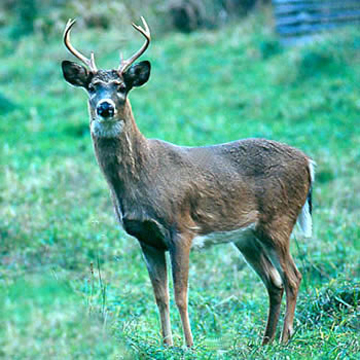
\includegraphics[width=0.6\textwidth, height=8cm]{imagenes/venado.jpg}
\caption{Venado de cola blanca}
\end{figure}



\endinput 